\documentclass[12pt]{report} 
\usepackage[
a4paper,
top=2.54cm,
bottom=2.54cm,
left=2.54cm,
right=2.5cm
]{geometry}


\usepackage[utf8]{inputenc}
\usepackage[T1]{fontenc}
\usepackage[spanish,activeacute]{babel}
\usepackage{url}

\usepackage{amsmath, graphicx}
\usepackage{indentfirst}
\usepackage{tabularx}
\usepackage{booktabs}  
\usepackage{makecell}  
\usepackage{multirow}  
\usepackage{array}   
\usepackage{tikz}
\usetikzlibrary{calc}               
\usepackage{helvet}
\usepackage{float}
\usepackage{longtable}
\usepackage[style=authoryear, backend=biber]{biblatex}
\usepackage[colorlinks=true, citecolor=black, linkcolor=black]{hyperref}
\usepackage{fancyhdr}
\usepackage{amssymb}
\pagestyle{fancy}
\fancyhf{}
% Define el encabezado: izquierda el documento, derecha el autor
\lhead{\footnotesize Liber: sistema software de gestión bibliotecaria}
\rhead{\footnotesize Manuel Martín Castelao}
\renewcommand{\headrulewidth}{0pt}
%pie de página con el número de página centrado
\cfoot{\thepage}
\addbibresource{referencias.bib}
\includeonly{capitulo4}

\begin{document}
	
	\begin{titlepage}
		\begin{tikzpicture}[remember picture, overlay]
			\draw[line width = 2pt] ($(current page.north west) + (1in,-1in)$) rectangle ($(current page.south east) + (-1in,1in)$);
		\end{tikzpicture}
		
		\begin{figure}[htb]
			\centering
			%\hspace{1.cm}
			
\includegraphics[width=4.5cm]{imagenes/UVA.png}
		\end{figure}
		
		\centering
		%\hspace{1.cm}
		{\fontfamily{phv}\selectfont{\large \textbf{Universidad de Valladolid}}}
		
		\vspace*{3cm}
		\centering
		%\hspace{1.cm}
		{\fontfamily{phv}\selectfont{\Large \textbf{ESCUELA DE INGENIER\'{I}A INFORM\'{A}TICA \\ 
					\vspace{.2cm}
					%\hspace{1.cm}
					DE SEGOVIA}}}
		
		\vspace*{0.5cm}
		%\hspace{1.cm}
		{\fontfamily{phv}\selectfont{\Large \textbf{Grado en Ingenier\'{\i}a Inform\'{a}tica \\ 
					%\hspace{1.cm}
					de Servicios y Aplicaciones}}}
		
		\vspace*{2cm}
		~\hspace{.5cm}\rule{140mm}{0.1mm}\\
		\vspace*{1cm}
		%\hspace{1.cm}
		{\fontfamily{phv}\selectfont{\Large \textbf{Liber: sistema software de gestión bibliotecaria}}}
		
		\vspace*{1.5cm}
		~\hspace{.5cm}\rule{140mm}{0.1mm}\\
		
		\vspace{.5cm}
		\raggedleft
		\vfill
		{\fontfamily{phv}\selectfont{\large \textbf{Alumno: Manuel Martín Castelao~\hspace{.5cm}}}}
		
		\vspace*{.5cm}
		{\fontfamily{phv}\selectfont{\large \textbf{Tutor: Fernando Díaz Gómez~\hspace{.5cm}}}}
		
	\end{titlepage}
	
	%% PAGINA EN BLANCO %% 
	\newpage 
	\thispagestyle{empty}
	$\,$
	
	
	\newpage
	{\LARGE APUNTE TEMPORAL SOBRE EL ÍNDICE} \\
	El índice se va a componer de tantos capítulos como apartados sean necesarios para tanto satisfacer las necesidades de información del proyecto y planificación como del producto en sí.
	La primera mitad de este documento contendrá información relativa al proyecto desde un punto de vista más integrador, como la planificación, contexto, etcétera, mientras que la segunda parte consistirá en temas más técnicos como la documentación técnica, que tendrá información sobre CÓMO se ha hecho el software. La primera mitad es técnica y la segunda tecnología. Más tarde, se verá si poner conclusiones por apartado teórico o solamente un capítulo más al final. Como anexo, se adjuntará el manual de usuario, o puede que sea otro capítulo, está por ver.
	
	% índice
	\tableofcontents
	
	\listoffigures
	\listoftables
	% --- capítulo1.tex ---

\chapter{Introducción}

% ===== CONTENIDO REAL DEL CAPÍTULO =====

\section{Estructura del documento (COMPLETAR CUANDO ESTÉ LA DOCUMENTACIÓN)}
En esta sección se encuentran los contenidos de este documento. Aquí se resume brevemente el objetivo de cada uno de los capítulos que lo componen, de modo que el lector pueda anticipar el contenido y la organización de la memoria.
\begin{itemize}
	\item \textbf{Capítulo 1 - Descripción del proyecto:} Se introduce la aplicación, acotando su alcance funcional, perfiles de usuario y restricciones de diseño para bibliotecas medianas y pequeñas. Asimismo, establece los objetivos del proyecto y su trazabilidad mediante la definición detallada de sus criterios de aceptación.
\end{itemize}

\section{Prólogo}
Las bibliotecas han desempeñado un papel fundamental en múltiples sociedades a lo largo de la historia. Durante siglos, estas han actuado como fuentes primarias de conocimiento al servicio de la humanidad. El concepto de la biblioteca —y sus derivados— ha funcionado como un arca del saber y la memoria colectiva a través del tiempo.

Antes, todo trabajo relacionado con la documentación implicaba una tarea compleja: las bibliotecas no eran sencillas de mantener, y su creación demandaba un nivel de organización y recursos que solo podían asumir grupos amplios y estructurados de personas. No obstante, gracias al desarrollo e integración de herramientas computacionales, construir un sistema de catalogación resulta hoy relativamente accesible. De hecho, desde hace décadas existen programas diseñados para cubrir las distintas necesidades que surgen en la gestión de una biblioteca —aspecto que se abordará en secciones posteriores—.

No obstante, estos sistemas pueden llegar a ser difícilmente comprensibles o aplicables a casos en los que tenemos una biblioteca con un fondo más reducido, dado que los sistemas de gestión de bibliotecas suelen estar preparados para ser escalables y contener una cantidad muy grande de información con la que trabaja una biblioteca, tales como datos de usuarios, ejemplares o préstamos. Las soluciones planteadas por la industria informática tienden a ofrecer recursos de —valga la redundancia— medidas industriales.

No todas las bibliotecas tienen el mismo tamaño, ni el mismo sujeto, ni por tanto las mismas necesidades. El sistema que se presenta en este proyecto está orientado a bibliotecas cuyo fondo es de tamaño mediano-pequeño. Debido a ello, será un sistema de gestión destinado a ser accesible, manejable, robusto y seguro en los entornos necesarios.

Una biblioteca no solamente presta a sus socios libros y recursos, sino que sirve de centro de documentación y archivo. Su propósito fundamental es conservar las ideas a lo largo del tiempo y hacer que la información sea pública y accesible para todos sus socios. 

Siguiendo esta línea de pensamiento, he tomado la decisión de desarrollar este proyecto manteniendo estos principios de accesibilidad y apertura. Es por ello por lo que este software será liberado bajo la Licencia Pública General de GNU (GPL), por lo que cualquier persona será libre de usarlo, modificarlo y distribuirlo libremente. De esta forma, cualquier institución o persona podrá apoyarse en este sistema para implementar una biblioteca de las características descritas, o adaptarlo a sus propias necesidades.

En relación con este enfoque de apertura y el dominio funcional del sistema, la aplicación web ha sido bautizada bajo la denominación de Liber. Este nombre responde a un doble propósito conceptual derivado de su etimología en latín, donde el término convive simultáneamente con dos acepciones esenciales para el proyecto: por un lado, hace referencia directa al "libro" \ como unidad primordial del catálogo que se gestiona y, por otro, evoca la condición de "libre", alineándose con el carácter de código abierto del software.

El presente documento constituye la memoria de mi Trabajo de Fin de Grado. En este se recogen de manera estructurada todos los aspectos relacionados con el desarrollo del sistema.

\section{Motivación}

Este proyecto encuentra su motivación fundamental en la preservación de la información y, por extensión, del conocimiento. La observación directa del funcionamiento de bibliotecas que no dependen de entidades gubernamentales ni de grandes instituciones deja ver una problemática cada vez más real: los sistemas de gestión disponibles ofrecen, generalizadamente, un rendimiento insuficiente o una complejidad desproporcionada para su implantación. Las bibliotecas más pequeñas o gestionadas por equipos reducidos necesitan, por tanto, un sistema de catalogación accesible y gratuito que les permita desempeñar su labor. Es precisamente el cubrir esta necesidad la que motiva el desarrollo del presente trabajo. 

\section{Objetivos generales del trabajo}

El fin de este Trabajo de Fin de Grado consiste en liberar un sistema de gestión de bibliotecas de fondo mediano o pequeño accesible para toda la comunidad, tanto para utilizarlo como para poder modificarlo, generando así una comunidad destinada al mantenimiento y posible ampliación de este sistema.  Este sistema ha sido concebido para ser fácil de entender e implementar, con el objeto de hacer la información y el tratamiento de la misma lo más accesible y manejable posible.

El proyecto desarrollado será destinado a bibliotecas cuyo fondo no sea demasiado grande; será una aplicación contenerizada que se podrá desplegar fácilmente para ser ejecutada en local o la nube; esa decisión será competencia de quien utilice el sistema. Una vez desplegada, se podrá usar para hacer tareas de gestión desde el lado de los bibliotecarios y responsables, para funciones tales como dar de alta (o baja) ejemplares, socios, hacer préstamos, y más acciones en las que se ahondará más adelante. También podrán hacer uso de esta aplicación los socios de la biblioteca; podrán usarla para consultar el catálogo disponible, solicitar un préstamo o darse de alta, por ejemplo. Por supuesto, habrá funciones adicionales para usuarios de tipo administrador, como poder hacer operaciones CRUD sobre toda la base de datos.

La aplicación se ha implementado con Django, un framework basado en Python, aprovechando la sencillez que este entorno ofrece para el desarrollo. Dicha elección busca facilitar la comprensión del código fuente, priorizando la legibilidad —dado que el software se liberará bajo una licencia libre— sobre la eficiencia aislada o la complejidad funcional. Se presta así atención a la relación del usuario o programador con el sistema, aspirando a que cualquier persona con nociones básicas de Python y programación pueda comprender y extender esta aplicación sin grandes dificultades.

La finalidad de este proyecto se puede dividir en los siguientes objetivos:

\begin{table}[H]
	\centering
	\caption{Objetivos generales del Trabajo de Fin de Grado.}
	\label{tab:objetivos_generales}
	\begin{tabularx}{\textwidth}{l X}
		\toprule
		\textbf{ID Objetivo} & \textbf{Nombre Objetivo} \\
		\midrule
		\textbf{OBJ-01} & Diseñar una aplicación web que permita la catalogación y gestión de fondos bibliotecarios medianos-pequeños. \\
		\addlinespace
		\textbf{OBJ-02} & Implementar un sistema seguro y robusto de gestión de usuarios diferenciando tres roles de acceso principales bien definidos; socios, bibliotecarios y administradores. \\
		\addlinespace
		\textbf{OBJ-03} & Automatizar el ciclo de vida de los préstamos, controlando las fechas de inicio, fin, devoluciones, prórrogas y la aplicación de penalizaciones por retraso. \\
		\addlinespace
		\textbf{OBJ-04} & Garantizar tanto la portabilidad como inmutabilidad del sistema mediante la contenerización completa de la aplicación recurriendo a Docker, facilitando el despliegue tanto localmente como en la nube. \\
		\addlinespace
		\textbf{OBJ-05} & Fomentar el software libre y la creación de comunidades de desarrollo mediante la liberación del código fuente bajo la Licencia Pública General de GNU (GPL), priorizando la legibilidad y simplicidad del código. \\
		\addlinespace
		\textbf{OBJ-06} & Consolidar a nivel personal las competencias adquiridas en el transcurso del grado en ingeniería, específicamente en el diseño de bases de datos relacionales, arquitectura de software por capas y despliegue de aplicaciones. \\
		\bottomrule
	\end{tabularx}
\end{table}


Más adelante, en el siguiente capítulo, se expondrán los criterios de aceptación para cada uno de los objetivos generales definidos.


\section{Alcance de la aplicación}
En esta sección se procede a definir los límites de la aplicación; todo aquello 
que se ha dejado tanto dentro como fuera de la misma. Se distingue entre el 
alcance del producto (qué funcionalidades ofrece Liber) y el alcance del 
proyecto (bajo qué condiciones se ha desarrollado).

\subsection{Alcance del producto: funcionalidades incluidas}
La aplicación Liber ha sido ideada para responder a las 
necesidades de gestión y catalogación de las bibliotecas de fondo 
mediano-pequeño, tales como las que podemos encontrar en colegios, 
asociaciones o centros culturales.

Con el fin de delimitar la interacción con el sistema, se han definido los 
siguientes perfiles de usuario atendiendo a su grado de especialización técnica:

\begin{itemize}
	\item \textbf{Personal técnico y operativo (Bibliotecarios y Administradores):}
	Este tipo de usuarios constituyen el núcleo de la gestión de Liber. Dado que interactuarán de manera directa con los módulos de catalogación, control de inventario y el ciclo de vida de los préstamos, se asume que estos usuarios poseen un conocimiento previo de los fundamentos sobre los sistemas de gestión bibliotecaria. Las interfaces destinadas a estos roles priorizan la eficiencia, la integridad de los datos y el acceso a operaciones CRUD complejas.
	
	\item \textbf{Usuarios finales (Socios):} 
	Representan a la comunidad que consume los recursos de la biblioteca. Al no precisar de competencias en biblioteconomía ni estar familiarizados con la catalogación, se les ofrece una interfaz intencionadamente simplificada. El alcance funcional para este perfil se restringe a acciones intuitivas y esenciales, tales como la consulta del catálogo público, la solicitud de reservas y la gestión de su perfil personal.
\end{itemize}

De una forma más concreta, las funcionalidades contempladas dentro del alcance 
del producto son las siguientes:

\begin{itemize}
	\item \textbf{Gestión del catálogo:} alta, modificación, consulta y baja de 
	obras y sus ejemplares físicos asociados.
	\item \textbf{Gestión de socios:} registro de usuarios, asignación de roles 
	(socio, bibliotecario, administrador) y control de penalizaciones.
	\item \textbf{Gestión de préstamos:} registro de préstamos, cálculo automático 
	de fechas de devolución, gestión de prórrogas y penalizaciones por retraso.
	\item \textbf{Catálogo público (OPAC):} consulta y búsqueda del fondo 
	bibliográfico por parte de socios y personal.
	\item \textbf{Despliegue contenerizado:} sistema desplegable mediante Docker, 
	tanto en local como en la nube.
	\item \textbf{Software libre:} liberación del código bajo licencia GPL v3 con 
	documentación que facilite su comprensión y extensión.
\end{itemize}

En última instancia, el propósito comercial y social de Liber es captar la 
atención de administradores, responsables de TI y personal directivo de 
organizaciones que busquen una solución de catalogación robusta, 
eficiente y alineada con la filosofía del software libre.

\subsection{Fuera del alcance: funcionalidades excluidas}
Con el objeto de acotar las expectativas del lector y evitar ambigüedades, 
se listan a continuación las funcionalidades que deliberadamente no forman 
parte de este Trabajo de Fin de Grado:

\begin{itemize}
	\item \textbf{Gestión de recursos electrónicos (ERM):} Liber se centra en 
	fondos físicos. La gestión de licencias de publicaciones electrónicas o 
	plataformas SaaS queda fuera del alcance.
	\item \textbf{Interoperabilidad con estándares bibliotecarios avanzados:} no 
	se implementa la importación ni exportación en formato MARC21/UNIMARC, dado 
	que las bibliotecas objetivo no lo requieren.
	\item \textbf{Préstamo interbibliotecario (ILL):} no se contempla la conexión 
	con redes de bibliotecas ni el intercambio de fondos entre instituciones.
	\item \textbf{Inteligencia artificial:} no se incluyen asistentes de 
	catalogación automática, recomendaciones ni analíticas avanzadas.
	\item \textbf{Aplicación móvil nativa:} la interfaz es web y adaptable, pero 
	no se desarrolla una app específica para dispositivos móviles.
	\item \textbf{Internacionalización completa:} la interfaz y documentación se ofrecen
	inicialmente en español, sin traducción a otros idiomas.
	\item \textbf{Módulo de adquisiciones y presupuestos:} no se gestionan 
	compras, proveedores ni facturación.
\end{itemize}

Estas funcionalidades, aunque presentes en soluciones de mayor envergadura 
como Koha o Alma, no resultan necesarias para el nicho de bibliotecas al que 
se orienta Liber, y su inclusión habría desviado el foco del proyecto.

\subsection{Alcance del proyecto: condicionantes}
Desde el punto de vista del proyecto y no del producto, el alcance de este 
Trabajo de Fin de Grado está condicionado por:

\begin{itemize}
	\item \textbf{Desarrollo individual:} el proyecto ha sido desarrollado por 
	un único alumno, bajo la supervisión del tutor.
	\item \textbf{Limitación temporal:} el desarrollo se ha ajustado a la 
	duración establecida.
	\item \textbf{Recursos técnicos:} se han empleado exclusivamente 
	herramientas de software libre (Django, PostgreSQL, Docker, Git).
\end{itemize}

Con el objeto de esclarecer visualmente las particularidades del proyecto, 
se presenta a continuación un árbol de características, que permite hacerse 
a la idea de lo que será y no será el producto resultante de este trabajo.

\begin{figure}[H]
	\centering
	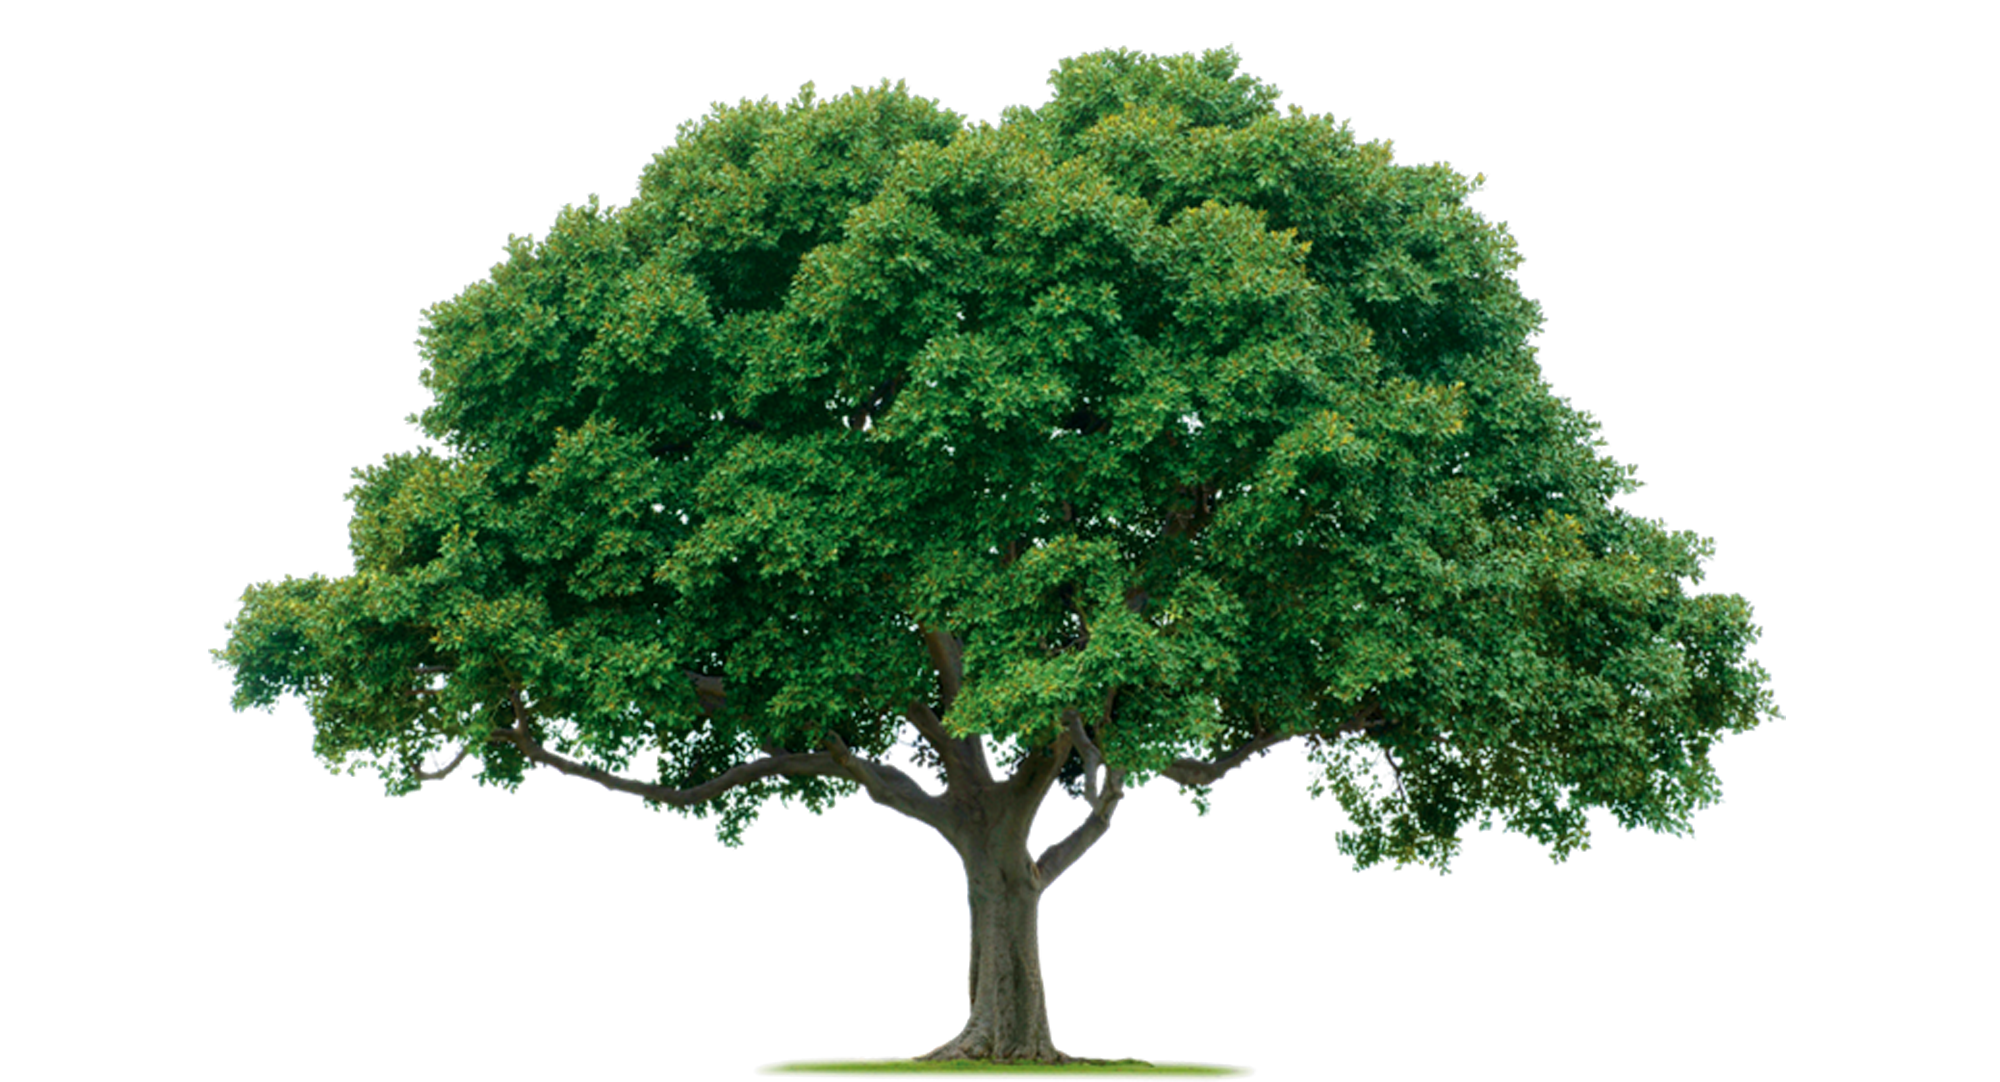
\includegraphics[width=\textwidth]{imagenes/arbol_caracteristicas.png}
	\caption{Árbol de características de Liber.}
	\label{fig:arbol_caracteristicas}
\end{figure}


\subsection{Definición de siglas y abreviaturas}
En este apartado se procede a definir una serie de siglas y expresiones utilizadas para abreviar con el objeto de que la experiencia del lector sea algo más ágil, incluso para aquel que no esté familiarizado con el léxico usado en la memoria.

\begin{table}[H]
	\centering
	\caption{Siglas y abreviaturas empleadas en la memoria.}
	\label{tab:siglas_abreviaturas}
	\begin{tabularx}{\textwidth}{l X}
		\toprule
		\textbf{Sigla / Abreviatura} & \textbf{Significado} \\
		\midrule
		ACID & Atomicity, Consistency, Isolation, Durability (Atomicidad, Consistencia, Aislamiento y Durabilidad) \\
		\addlinespace
		API & Application Programming Interface (Interfaz de Programación de Aplicaciones) \\
		\addlinespace
		CI/CD & Continuous Integration / Continuous Delivery (Integración Continua / Entrega Continua) \\
		\addlinespace
		CRUD & Create, Read, Update, Delete (Crear, Leer, Actualizar, Eliminar) \\
		\addlinespace
		DRY & Don't Repeat Yourself (No te repitas) \\
		\addlinespace
		EAN & European Article Number (Número de Artículo Europeo) \\
		\addlinespace
		ERM & Electronic Resource Management (Gestión de Recursos Electrónicos) \\
		\addlinespace
		GPL & GNU General Public License (Licencia Pública General de GNU) \\
		\addlinespace
		IA & Inteligencia Artificial \\
		\addlinespace
		ILL & Interlibrary Loan (Préstamo Interbibliotecario) \\
		\addlinespace
		ILS & Integrated Library System (Sistema Integrado de Gestión Bibliotecaria) \\
		\addlinespace
		ISBN & International Standard Book Number (Número Internacional Normalizado de Libros) \\
		\addlinespace
		JSON & JavaScript Object Notation (Notación de Objetos de JavaScript) \\
		\addlinespace
		MARC & Machine-Readable Cataloging (Catalogación Legible por Máquina) \\
		\addlinespace
		MVT & Model-View-Template (Modelo-Vista-Plantilla) \\
		\addlinespace
		OPAC & Online Public Access Catalog (Catálogo Público de Acceso en Línea) \\
		\addlinespace
		ORM & Object-Relational Mapping (Mapeo Objeto-Relacional) \\
		\addlinespace
		PSB & Plataforma de Servicios Bibliotecarios \\
		\addlinespace
		SaaS & Software as a Service (Software como Servicio) \\
		\addlinespace
		SIGB & Sistema Integrado de Gestión Bibliotecaria \\
		\addlinespace
		SQL & Structured Query Language (Lenguaje de Consulta Estructurado) \\
		\addlinespace
		TFG & Trabajo de Fin de Grado \\
		\addlinespace
		UML & Unified Modeling Language (Lenguaje Unificado de Modelado) \\
		\addlinespace
		WMS & WorldShare Management Services \\
		\bottomrule
	\end{tabularx}
\end{table}
	\chapter{Contexto del proyecto}
En este capítulo se tratarán tanto los antecedentes como el estado del arte. Primeramente se expondrán los diferentes tipos de software de gestión bibliotecaria, así como su evolución. Tras ello, se explicarán brevemente las soluciones software de gestión de bibliotecas, y se describirán tanto sus ventajas como sus inconvenientes. Una vez explicadas las particularidades de cada sistema software en el estado del arte, se hará una breve comparativa de estas tecnologías con Liber. Para finalizar el capítulo, se expondrán las tecnologías utilizadas; tanto sus características como la motivación de usarlas.

\section{Antecedentes: evolución histórica de los sistemas de gestión bibliotecaria}

La gestión automatizada de bibliotecas no es un fenómeno reciente, es el resultado de una evolución tecnológica y conceptual que comienza hace más de medio siglo. Comprender su trayectoria es fundamental para situar el presente proyecto en su contexto y valorar las decisiones de diseño adoptadas durante el desarrollo.

Los orígenes de la automatización bibliotecaria mediante computación se remontan a la década de 1960, con iniciativas pioneras como el desarrollo del protocolo MARC (\textit{Machine-Readable Cataloging}) por parte de la Biblioteca del Congreso de Estados Unidos. Este estándar, que permitía el intercambio de registros bibliográficos en formato legible por máquina, estableció las bases para la creación de los primeros catálogos automatizados y marcó un hito en la estandarización de los datos bibliográficos mundialmente. La adopción de MARC facilitó la colaboración entre instituciones y creación de redes bibliotecarias, transformando profundamente los procesos de catalogación y descripción de fondos.

Entre las décadas de 1970 y 1980, los sistemas de gestión bibliotecaria experimentaron un desarrollo significativo con la aparición de los primeros ILS (\textit{Integrated Library Systems}), o SIGB (Sistemas Integrados de Gestión Bibliotecaria), en español. Estas plataformas, inicialmente concebidas para entornos \textit{mainframe}, integraban funcionalidades básicas tales como catálogos en línea, control de préstamos y adquisiciones. No obstante, se trataba de sistemas propietarios, con un coste elevado y una complejidad técnica que limitaba su rango de implantación a grandes bibliotecas universitarias y nacionales. El estudio \textit{Library Management Systems Study} \parencite{jisc2008} ofrece una panorámica detallada de este periodo, identificando los principales sistemas comerciales y sus capacidades, así como las limitaciones derivadas de su arquitectura monolítica y su escasa flexibilidad. Los sistemas integrados de gestión bibliotecaria, al igual que los recursos computacionales, era algo que solamente cierto tipo de organizaciones podía permitirse implementar durante estas décadas en las que la computación aún era algo complejo de comprender y costoso de implementar.

La consolidación del mercado de sistemas de gestión bibliotecaria en las décadas de 1990 y 2000 vino acompañada de una intensa actividad de fusiones y adquisiciones empresariales. Breeding \parencite{breeding_history} documenta gráficamente este proceso, mostrando cómo numerosos proveedores independientes fueron absorbidos por grandes conglomerados, reduciendo la diversidad del mercado y consolidando un puñado de soluciones dominantes. Este suceso, aunque permitió la integración de funcionalidades y la creación de plataformas más completas, también generó una fuerte dependencia de unos pocos proveedores y dificultó la aparición de alternativas más flexibles o adaptadas a contextos específicos; a cambio de tener unos estándares centralizados, había pocas alternativas.

A finales de la primera década del siglo XXI, el panorama de los sistemas de gestión bibliotecaria comenzó a diversificarse con la aparición de soluciones de código abierto, siendo Koha (2000) y Evergreen (2006) los exponentes más destacados. La creación de este tipo de plataformas de catalogación de código abierto surge como respuesta a la necesidad de establecer ciertos estándares de comunicación y almacenamiento de información, dado que previamente solo había complejos sistemas originados en organizaciones de gran extensión. Durante estos años, estos sistemas de catalogación se comienzan a poner al servicio de clientes más de a pie, a usuarios menos experimentados, usando tecnologías de este tipo. Estas plataformas ofrecían una alternativa a los sistemas propietarios, con modelos de desarrollo colaborativo que permitían una mayor personalización y un coste de adquisición reducido. Sin embargo, la complejidad de su implantación y mantenimiento seguía siendo un obstáculo para bibliotecas de menor tamaño. Paralelamente, la web 2.0 y el desarrollo de tecnologías como los OPACs de nueva generación transformaron las expectativas de los usuarios, que demandaban interfaces más intuitivas y funcionalidades sociales.

Asimismo, la evolución de las publicaciones hacia formatos electrónicos trajo consigo la necesidad de una gestión distinta de los recursos. Surgen así las Plataformas de Servicios Bibliotecarios (PSB), también denominadas SIGB de nueva generación. Como señala Sandra Cano \parencite{cano2021psb} en su trabajo fin de grado, \textit{``las PSB nacen de la necesidad de unificar los tradicionales flujos de trabajos de las bibliotecas con las nuevas necesidades tecnológicas de los documentos electrónicos''}. La principal razón de ser de las PSB es gestionar de manera integrada tanto materiales impresos como electrónicos, consolidando en un único sistema funciones que antes requerían de múltiples productos especializados.

Marshall Breeding estimó que para 2020 las bibliotecas académicas o de investigación usarían PSB y para 2026 serían todas las bibliotecas \parencite{breeding_history}. La principal razón por la que se pueda retrasar el acercamiento de las plataformas en las bibliotecas es debido al coste económico que supone implementar un nuevo sistema, sustituyendo a uno que ya funciona a pesar de las posibles limitaciones que tenga, y más cuando es la novedad en el mercado de los softwares de bibliotecas.

Las PSB se caracterizan por \parencite{cano2021psb}:
\begin{itemize}
	\item Relacionar los módulos entre sí (por ejemplo, asignar un usuario en concreto para un préstamo, relacionando los módulos de gestión de usuarios con el de préstamos).
	\item Utilizar una única base de datos para gestionar todas las funciones.
	\item Automatizar los procesos.
\end{itemize}

Entre las principales PSB del mercado destacan Alma (de Ex Libris, propiedad de ProQuest), Sierra (de Innovative Interfaces), y WorldShare Management Services (de OCLC). A diferencia de los SIGB tradicionales, que se adquirían mediante compra de licencia, las PSB se ofrecen bajo modelo de suscripción o de software como servicio (SaaS, Software as a Service) con precios que varían según el tamaño de almacenamiento y las funcionalidades contratadas. Además, su arquitectura \textit{multi-tenant} y basada en la nube permite a las bibliotecas acceder al sistema desde cualquier dispositivo sin necesidad de instalación local, con actualizaciones globales aplicadas por el proveedor, y con APIs expuestas que facilitan la interoperabilidad con otros sistemas.

En este contexto, el proyecto \textit{HeLibTech} \parencite{helibtech} surge como un recurso colaborativo para la comunidad de educación superior en el Reino Unido, manteniendo actualizada la información sobre el ecosistema tecnológico bibliotecario. Su enfoque comunitario y su vocación de servicio público reflejan una tendencia creciente hacia la apertura y el intercambio de conocimiento en el ámbito de la tecnología bibliotecaria, una filosofía que el presente trabajo de fin de grado comparte y promueve.

La evolución histórica evidencia que, a pesar de los avances, persisten desafíos importantes. Muchos de los sistemas actuales, tanto comerciales como de código abierto, mantienen una complejidad inherente que los hace difíciles de desplegar y mantener por personal sin una formación técnica especializada. Asimismo, la tendencia hacia soluciones monolíticas o excesivamente modulares no siempre se traduce en una experiencia de usuario satisfactoria o en una gestión eficiente para bibliotecas de dimensiones reducidas. Es en este punto donde se enmarca la propuesta del presente trabajo: el desarrollo de un sistema de gestión de bibliotecas basado en Docker que, inspirándose en las lecciones del pasado y en las tecnologías más actuales, ofrezca una alternativa sencilla, liviana y fácilmente comprensible para bibliotecas medianas y pequeñas, con un fuerte énfasis en la accesibilidad y la apertura.

\section{Estado del arte}
Recogiendo lo expuesto en los antecedentes, se puede entrever el panorama actual de las soluciones software para bibliotecas.

Hoy en día se pueden identificar dos corrientes claras; los SIGB tradicionales y las Plataformas de Servicios Bibliotecarios (PSB) más modernas. La información muestra que, pese a que los SIGB dominen en número de instalaciones, el futuro está marcado por la inteligencia artificial y la nube, herramientas características de las PSB.

Es por esto por lo que podemos decir que nos encontramos en un punto de inflexión en lo que a soluciones software para bibliotecas se refiere. Observamos un mercado maduro y marcado tradicionalmente por grandes corporaciones o agrupaciones colaborativas que día a día está siendo redefinido por las nuevas plataformas \parencite{americanlibraries2026}. Al igual que ocurre en otros muchos ámbitos relacionados con las soluciones software, los sistemas bajo licencia están dando paso a modelos bajo suscripción. Más específicamente en el ámbito de estos sistemas de gestión, se podría decir que se está pasando de una forma de gestionar la biblioteca mediante diferentes tecnologías o \textit{suites} por licencia, a un modelo más unificado, hacia software más uniformizado o monolítico que cubre todas las funciones necesarias a través de una única suscripción.

Todas estas nuevas tecnologías permiten optimizar el funcionamiento de las bibliotecas que las integran a través de nuevas funcionalidades, como el uso de la inteligencia artificial o una instalación más sencilla a través de licencia. Al tratarse normalmente de servicios SaaS, se hace más fácil el uso e instalación de las PSB frente a los tradicionales SIGB.

Sin embargo, estas nuevas soluciones también presentan severas barreras de entrada, sobre todo para bibliotecas con poco personal técnico o medios económicos limitados \parencite{americanlibraries2026}. Este tipo de instituciones no pueden permitirse contratar administradores de sistemas dedicados a comprender el software, ni asumir el coste de una PSB. Es precisamente en este punto donde se enmarca la propuesta del presente trabajo.

Ahora que tenemos plataformas en la nube para gestionar la mayoría de bibliotecas, parece ser que estamos cerca de una coyuntura en la que la mayoría de bibliotecas tendrán un sistema de gestión moderno, integrado con inteligencia artificial, y que ofrezca nuevas funcionalidades tanto para usuarios como para el personal de la propia biblioteca. Nada más lejos de la realidad; en este sector, al igual que en la mayoría, nos podemos encontrar con una gran variedad de tipos de bibliotecas. No todas las bibliotecas pueden tener las mismas necesidades, sobre todo cuando entran en juego factores como a qué está orientada su funcionalidad, a qué clase de público quiere llegar, o el tamaño sin ir más lejos.
En este contexto cuasi trascendental, aparecen una serie de herramientas recientes que parecen estar marcando el futuro próximo de estos sistemas bibliotecarios, dado que son los PSB que más apuestan por la innovación.

\subsection{Alma}
\begin{figure}[htb]
	\centering
	
\includegraphics[scale=0.5]{imagenes/exlibris.jpg}
	\caption{Logo de Alma}
	\label{fig:alma}
\end{figure}
Alma es una plataforma de servicios bibliotecarios basada en la nube desarrollada por Ex Libris \parencite{exlibris_alma_platform}, adquirida primero por ProQuest, y más tarde por Clarivate en los últimos años, y actualmente es la plataforma principal utilizada por bibliotecas académicas y nacionales, implementada en más de 2700 instituciones en todo el mundo. Alma integra las funciones de los sistemas tradicionales de gestión bibliotecaria (SIGB) con la gestión de recursos electrónicos (ERM), adoptando un modelo de Software como Servicio (SaaS) y arquitectura multi-inquilino, donde la infraestructura del servidor, el mantenimiento de la base de datos y las actualizaciones de software son gestionados por Ex Libris.

La hoja de ruta que Alma \parencite{exlibris_alma_roadmap2026} pretende seguir en 2026 muestra que el enfoque de Alma hoy día mira hacia la IA, introduciendo asistentes inteligentes de metadatos para catalogación, adquisiciones y análisis.

Por una parte, Alma tiene una funcionalidad completa, cubriendo la gestión unificada de recursos físicos, electrónicos y digitales; su arquitectura SaaS reduce la carga de mantenimiento local; la IA mejora la eficiencia de catalogación y análisis, además de ofrecer soporte de red a nivel de consorcio para bibliotecas, permitiendo compartir la información entre las mismas.

Sin embargo presenta ciertas barreras de entrada: precio elevado, modelo de suscripción, funcionalidad compleja, con una curva de aprendizaje pronunciada. Depende de proveedores comerciales, con poca flexibilidad de personalización. Para bibliotecas con recursos técnicos y presupuestarios limitados, estas características componen un obstáculo.

\subsection{WorldShare Management Services}
\begin{figure}[htb]
	\centering
	
\includegraphics{imagenes/WMS.png}
	\caption{Logo de WorldShare Management Services}
\end{figure}

WorldShare Management Services (WMS por sus siglas) es la plataforma de servicios bibliotecarios en la nube de OCLC, cuya ventaja central radica en estar construida sobre WorldCat, la red global de datos bibliotecarios más grande del mundo. En los últimos 12 meses, 48 nuevas bibliotecas se han unido a la comunidad WMS \parencite{oclc_48nuevas2026}, incluyendo instituciones como Old Dominion University y la universidad de Medellín \parencite{oclc_odu2026}. WMS soporta las funciones principales de adquisiciones, circulación, catalogación, descubrimiento, préstamo interbibliotecario y gestión de licencias.

Es una herramienta muy útil ya que tiene integración con WorldCat, permitiendo el acceso a datos bibliográficos de cientos de millones de registros, la infraestructura compartida reduce el trabajo repetitivo, además de que está desarrollada por una organización sin ánimo de lucro, con precios relativamente razonables \parencite{oclc_wms_platform}.
Por otra parte, es cierto que es un ecosistema complejo pensado para bibliotecas que colaboran internacionalmente tales como las universidades mencionadas.

Queda claro que las PSB presentan soluciones muy prácticas para los casos de uso de las bibliotecas de hoy en día, brindando una alternativa a los clásicos SIGB a la vez que ofreciendo propiedades muy competitivas. Sin embargo, y recuperando lo mencionado previamente, este proyecto se encuentra en el nicho de las bibliotecas de fondo reducido, en el cual las bibliotecas no demandan una red de interconexión para compartir catálogos, ni se hacen necesarios asistentes de inteligencia artificial. A continuación se exponen ciertas soluciones existentes dentro de este mismo nicho; software de asistencia a la gestión de las bibliotecas más pequeñas o locales, con funcionalidades más sencillas o tradicionales, pero que por otra parte tienen un uso bastante extendido.

\subsection{Koha}
\begin{figure}[htb]
	\centering
	
\includegraphics[scale=0.5]{imagenes/koha.png}
	\caption{Logo de Koha}
	\label{fig:koha}
\end{figure}

Koha es el primer SIGB de código abierto del mundo. Se empezó a desarrollar en 1999 en Nueva Zelanda por el consorcio Horowhenua Library Trust. «Koha» proviene del maorí y significa «regalo» o «dar algo a la comunidad», reflejando la filosofía colaborativa que ha marcado el proyecto desde sus inicios. Está desarrollado y distribuido bajo la licencia GNU General Public License (GPL), por lo que garantiza a las bibliotecas la libertad de usar, modificar y distribuir el software sin restricciones \parencite{koha_zenodo2025}.

El \textit{stack} tecnológico de la herramienta está compuesto por Linux, Apache, MySQL/ MariaDB y Perl. Al igual que Liber, es una herramienta basada en web, tanto para el personal bibliotecario como para los usuarios finales, contribuyendo a que el sistema sea ligero, fácil de usar, desplegar y gestionar \parencite{koha_librarytechnology_ruskin2026}. Soporta una gran variedad de estándares, entre ellos MARC21 y UNIMARC, lo que facilita la compatibilidad con otros sistemas \parencite{koha_kohasupport2025}.

La modularidad es identitaria de Koha. El sistema incluye módulos integrados para catalogación, circulación, adquisiciones, gestión de publicaciones seriadas, OPAC, informes y gestión de usuarios. Un aspecto destacable es que todos los módulos esenciales vienen incluidos en la instalación básica sin coste adicional, lo que supone una ventaja significativa frente a los sistemas propietarios que suelen cobrar por módulos o funcionalidades específicas \parencite{koha_zenodo2025}.

Entre las principales ventajas de Koha encontramos la ausencia de costes de licencia, libertad para modificar el software según las necesidades de cada biblioteca, la ausencia de dependencia de un proveedor único y el respaldo de una comunidad global muy activa, en resumidas cuentas todas las ventajas que puede tener un software de licencia GPL bien mantenido. Su adopción es notable: según datos de 2026, Koha cuenta con más de 18.000 instalaciones en todo el mundo \parencite{koha_librarytechnology_ruskin2026}, y se utiliza en bibliotecas de todo tipo, desde pequeñas bibliotecas escolares hasta grandes consorcios universitarios y redes de bibliotecas públicas.

No obstante, Koha presenta limitaciones a considerar. Su instalación y mantenimiento requieren conocimientos técnicos en Linux, Apache y MySQL, así como acceso total al servidor \parencite{koha_zenodo2025, koha_sourceforge2026}. Aunque existen servicios de \textit{hosting} gestionado que reducen esta barrera, el despliegue autogestionado sigue siendo complejo para bibliotecas sin personal técnico especializado.

Koha es una solución madura, flexible y sostenible para bibliotecas que buscan un sistema completo sin costes de licencia, pero su adopción demanda cierta complejidad técnica. Para el nicho de bibliotecas que aborda este proyecto, Koha se sitúa en un punto intermedio: ofrece más funcionalidades de las necesarias para una biblioteca pequeña y exige un nivel de infraestructura y conocimientos técnicos que pueden resultar desproporcionados.

\subsection{OpenBiblio}
\begin{figure}[htb]
	\centering
	
\includegraphics{imagenes/openbiblio.png}
	\caption{Logo de OpenBiblio}
	\label{fig:openbiblio}
\end{figure}

OpenBiblio es un SIGB de código abierto, desarrollado en PHP y MySQL, y distribuido bajo la licencia GNU General Public License (GPL). Su objetivo principal es cubrir las necesidades de automatización de bibliotecas pequeñas, ofreciendo una herramienta sencilla que no requiere una infraestructura técnica compleja \parencite{bwalya2017openbiblio, openbiblio_docs}.

A diferencia de Koha, cuyo despliegue exige conocimientos avanzados de Linux, Apache y Perl, OpenBiblio está diseñado para ser fácil de instalar y configurar. La documentación oficial describe su instalación tanto en Windows como en Linux mediante entornos como EasyPHP o servidores compartidos, con requisitos mínimos.

El sistema se organiza en cuatro módulos que representan las funciones esenciales de una biblioteca pequeña: Catalogación, Circulación, OPAC y Gestión de Usuarios. Permite la importación de registros MARC y CSV, así como la catalogación manual \parencite{vimalkumar2005}.

La ventaja más importante de OpenBiblio radica en su simplicidad. No requiere personal técnico especializado para su puesta en marcha y mantenimiento, y su curva de aprendizaje es notablemente inferior a la de otras soluciones de código abierto. Sin embargo, la sencillez también implica limitaciones: carece de módulos avanzados como adquisiciones, control de publicaciones seriadas o gestión de recursos electrónicos, y su OPAC no es tan avanzado para búsquedas en comparación con sistemas más completos \parencite{vimalkumar2005}.

Otra desventaja señalada en la literatura es la escasez de documentación actualizada en Internet, lo que puede dificultar la resolución de problemas para usuarios \parencite{bwalya2017openbiblio}. No obstante, el proyecto mantiene una comunidad activa y dispone de documentación oficial accesible en GitHub, que cubre desde la instalación hasta la administración del sistema \parencite{openbiblio_docs}.

En el contexto de este proyecto, OpenBiblio representa el extremo opuesto del espectro: es la solución más ligera y accesible entre opciones de código abierto, pero su arquitectura (PHP/MySQL) y su limitado conjunto de funcionalidades no ofrecen la flexibilidad ni la modernidad que se buscan en una aplicación web contemporánea. Esto refuerza la necesidad de una alternativa que combine la simplicidad de OpenBiblio con las capacidades de un framework moderno como Django.

\subsection{Tabla comparativa}
Con el objeto de exponer más visualmente las principales diferencias entre las soluciones software expuestas, se ha elaborado una tabla que nombra las características de cada sistema en diferentes aspectos:
\newpage
\thispagestyle{empty}
\begin{table}[H]
	\vspace{-1cm}
	\centering
	\caption{Cuadro comparativo de las soluciones de gestión bibliotecaria analizadas.}
	\label{tab:comparativa_soluciones}
	\small
	\begin{tabularx}{\textwidth}{p{2.5cm} X X X X X}
		\toprule
		\textbf{Característica} & \textbf{Alma} & \textbf{WMS} & \textbf{Koha} & \textbf{OpenBiblio} & \textbf{Liber} \\
		\midrule
		
		\textbf{Tipo} & PSB comercial & PSB comercial & SIGB open source & SIGB open source & SIGB open source \\
		\addlinespace
		
		\textbf{Desarrollador} & Ex Libris (Clarivate) & OCLC & Comunidad Koha & Comunidad OpenBiblio & Proyecto propio \\
		\addlinespace
		
		\textbf{Licencia} & Propietaria & Propietaria & GPL & GPL & GPL \\
		\addlinespace
		
		\textbf{Modelo de despliegue} & SaaS & SaaS & Autoalojado o hosting gestionado & Autoalojado & Contenerizado (Docker) \\
		\addlinespace
		
		\textbf{Stack} & Propietario & Propietario & Linux, Apache, MySQL/MariaDB, Perl & PHP, MySQL & Python, Django, PostgreSQL \\
		\addlinespace
		
		\textbf{Requisitos técnicos} & Bajos & Bajos & Medios-altos & Bajos-medios & Bajos \\
		\addlinespace
		
		\textbf{Costes} & Suscripción elevada & Suscripción moderada & Sin licencia (costes de hosting) & Sin licencia (costes de hosting) & Sin licencia (costes de hosting)\\
		\addlinespace
		
		\textbf{Módulos principales} & Catalogación, circulación, adquisiciones, ERM, analíticas, descubrimiento & Adquisiciones, circulación, catalogación, descubrimiento, ILL, licencias & Catalogación, circulación, adquisiciones, seriadas, OPAC, informes & Catalogación, circulación, OPAC, usuarios & Catalogación, circulación, usuarios, OPAC \\
		\addlinespace
		
		\textbf{Gestión de recursos electrónicos} & Sí, nativa y avanzada & Sí, integrada & Parcial & No & No \\
		\addlinespace
		
		\textbf{Alcance} & Grandes consorcios y bibliotecas nacionales & Redes internacionales de bibliotecas & Desde pequeñas bibliotecas hasta grandes consorcios & Bibliotecas pequeñas & Bibliotecas medianas-pequeñas \\
		\addlinespace
		
		\textbf{Público objetivo} & Bibliotecas académicas y nacionales & Bibliotecas académicas y redes internacionales & Bibliotecas de cualquier tamaño & Bibliotecas pequeñas y rurales & Bibliotecas medianas-pequeñas \\
		\addlinespace
		
		\bottomrule
	\end{tabularx}
\end{table}

\newpage

\section{Tecnologías utilizadas}

Liber ha sido desarrollada utilizando Django como framework principal, junto con una serie de herramientas de apoyo para facilitar el desarrollo, las pruebas, el despliegue y la gestión del código.

A continuación, se enumeran las principales características de las tecnologías empleadas, divididas en backend, base de datos, herramientas de desarrollo y documentación.

\subsection{Backend}

\subsubsection{Django}
\begin{figure}[htb]
	\centering
	
\includegraphics[width=3cm]{imagenes/django.png}
	\caption{Logo de Django}
	\label{fig:django}
\end{figure}

Django es un \textit{framework} de desarrollo web de alto nivel escrito en Python. Sigue el patrón de diseño \textit{Modelo-Vista-Template} (MVT), muy similar al Modelo-Vista-Controlador, y promueve el principio DRY (\textit{Don't Repeat Yourself}), lo que facilita la creación de aplicaciones web robustas y mantenibles.

Características principales del \textit{framework}:
\begin{itemize}
	\item Framework completo con ORM integrado, sistema de autenticación, panel de administración y gestión de formularios.
	\item Arquitectura MVT que separa la lógica de negocio, la presentación y el acceso a datos.
	\item ORM que permite interactuar con la base de datos mediante código Python, sin escribir SQL manualmente.
	\item Sistema de migraciones que versiona los cambios en el esquema de la base de datos.
	\item Panel de administración autogenerado que facilita la gestión de los modelos de datos.
	\item Compatibilidad con múltiples bases de datos (PostgreSQL, MySQL, SQLite, etc.).
	\item Enrutamiento de URLs limpio y flexible mediante expresiones regulares o convertidores de ruta.
\end{itemize}

\subsection{Base de datos}

\subsubsection{PostgreSQL}
\begin{figure}[htb]
	\centering
	
\includegraphics[width=3cm]{imagenes/postgresql.png}
	\caption{Logo de PostgreSQL}
	\label{fig:postgresql}
\end{figure}

PostgreSQL es un sistema de gestión de bases de datos relacional de código abierto, conocido por su robustez, integridad y cumplimiento de estándares SQL.

Características principales:
\begin{itemize}
	\item Soporte completo de transacciones ACID.
	\item Integridad referencial mediante claves primarias, foráneas y restricciones.
	\item Soporte para tipos de datos avanzados (JSON, arrays, rangos, etc.).
	\item Escalabilidad y alto rendimiento en entornos de producción.
	\item Integración nativa con Django a través de su ORM.
\end{itemize}

\subsection{Herramientas de desarrollo}

\subsubsection{Visual Studio Code}
\begin{figure}[htb]
	\centering
	
\includegraphics[width=3cm]{imagenes/vscode.png}
	\caption{Logo de Visual Studio Code}
	\label{fig:vscode}
\end{figure}

Visual Studio Code es un editor de código fuente ligero pero potente, desarrollado por Microsoft, que se ha convertido en uno de los editores más utilizados en el desarrollo de software.

Características principales:
\begin{itemize}
	\item Soporte nativo para múltiples lenguajes de programación, incluido Python.
	\item Extensible mediante extensiones (Python, Django, Docker, Git, etc.).
	\item Terminal integrada que permite ejecutar comandos sin salir del editor.
	\item Depurador integrado para Python y otros lenguajes.
	\item Integración con Git y GitHub para control de versiones.
\end{itemize}

\subsubsection{Docker}
\begin{figure}[htb]
	\centering
	
\includegraphics[width=3cm]{imagenes/docker.png}
	\caption{Logo de Docker}
	\label{fig:docker}
\end{figure}

Docker es una plataforma de contenerización que permite empaquetar aplicaciones y sus dependencias en contenedores ligeros y portables, garantizando que se ejecuten de la misma forma en cualquier entorno.

Características principales:
\begin{itemize}
	\item Aislamiento de la aplicación y sus dependencias en contenedores.
	\item Portabilidad: el mismo contenedor funciona en desarrollo, pruebas y producción.
	\item Definición de la infraestructura como código mediante \texttt{Dockerfile} y \texttt{docker-compose.yml}.
	\item Compatibilidad de despliegue en la mayoría de servidores o servicios en la nube.
	\item Reducción de conflictos entre entornos de desarrollo y producción.
\end{itemize}

\subsubsection{Git y GitHub}

\begin{figure}[htb]
	\centering
	\begin{minipage}{0.45\textwidth}
		\centering
		
\includegraphics[width=3cm]{imagenes/git.png}
		\caption{Logo de Git}
		\label{fig:git}
	\end{minipage}
	\hfill
	\begin{minipage}{0.45\textwidth}
		\centering
		
\includegraphics[width=3cm]{imagenes/github.png}
		\caption{Logo de GitHub}
		\label{fig:github}
	\end{minipage}
\end{figure}

Git es un sistema de control de versiones distribuido que permite registrar los cambios en el código y colaborar con otros desarrolladores. GitHub es una plataforma basada en Git que permite alojar y gestionar repositorios de código de forma remota y colaborativa.

Características principales:
\begin{itemize}
	\item Control de versiones distribuido que evita pérdidas de código y permite revertir cambios.
	\item Trabajo con ramas para desarrollar funcionalidades de forma segura sin afectar a la versión principal.
	\item Fusión de ramas (\textit{merge}) y resolución de conflictos.
	\item Gestión de \textit{issues} y \textit{pull requests} en GitHub.
	\item Histórico completo de cambios y aportaciones.
	\item Integración con CI/CD para automatización de pruebas y despliegues.
\end{itemize}

\subsubsection{pgAdmin}
\begin{figure}[htb]
	\centering
	
\includegraphics[width=3cm]{imagenes/pgadmin.png}
	\caption{Logo de pgAdmin}
	\label{fig:pgadmin}
\end{figure}

pgAdmin es una herramienta gráfica de administración para PostgreSQL que permite gestionar bases de datos, ejecutar consultas y visualizar datos sin necesidad de utilizar la línea de comandos.

Características principales:
\begin{itemize}
	\item Interfaz visual intuitiva para la gestión de bases de datos.
	\item Editor SQL con resaltado de sintaxis y autocompletado.
	\item Visualización de datos en tablas y exportación en varios formatos.
	\item Gestión de usuarios, roles y permisos.
	\item Monitorización del rendimiento y de las consultas ejecutadas.
\end{itemize}

\subsection{Documentación}

\subsubsection{LaTeX}
\begin{figure}[htb]
	\centering
	
\includegraphics[width=3cm]{imagenes/latex.png}
	\caption{Logo de LaTeX}
	\label{fig:latex}
\end{figure}

LaTeX es un sistema de composición de documentos de alta calidad, ampliamente utilizado en el ámbito académico y científico para la redacción de tesis, artículos y memorias.

Características principales:
\begin{itemize}
	\item Composición tipográfica profesional y consistente.
	\item Gestión automática de índices, referencias cruzadas y bibliografía.
	\item Separación entre contenido y formato, lo que facilita el mantenimiento del documento.
	\item Amplia variedad de paquetes para tablas, figuras, código fuente y matemáticas.
	\item Ideal para documentos extensos como memorias de TFG.
\end{itemize}

\subsubsection{TeXstudio}
\begin{figure}[htb]
	\centering
	
\includegraphics[width=3cm]{imagenes/texstudio.png}
	\caption{Logo de TeXstudio}
	\label{fig:texstudio}
\end{figure}

TeXstudio es un editor de código abierto específicamente diseñado para trabajar con LaTeX. Proporciona un entorno integrado que facilita la escritura, compilación y visualización de documentos LaTeX, con funcionalidades pensadas para agilizar el trabajo con documentos extensos.

Características principales:
\begin{itemize}
	\item Editor con resaltado de sintaxis específico para LaTeX.
	\item Autocompletado de comandos, entornos y referencias bibliográficas.
	\item Visor de PDF integrado con sincronización entre el código fuente y el documento compilado.
	\item Gestión de la estructura del documento mediante un árbol de secciones, figuras, tablas y etiquetas.
	\item Configuración de la cadena de compilación (PdfLaTeX, Biber, etc.) y detección automática de errores.
	\item Integración con Git y otros sistemas de control de versiones.
\end{itemize}

\subsubsection{draw.io}
\begin{figure}[htb]
	\centering
	
\includegraphics[width=3cm]{imagenes/drawio.png}
	\caption{Logo de draw.io}
	\label{fig:drawio}
\end{figure}

draw.io es una herramienta de diagramación de código abierto que permite crear diagramas de flujo, diagramas entidad-relación, diagramas UML y esquemas de arquitectura de software de forma visual e intuitiva.

Características principales:
\begin{itemize}
	\item Interfaz gráfica basada en arrastrar y soltar, sin necesidad de escribir código.
	\item Amplia biblioteca de formas y plantillas para diagramas UML, ER, redes, arquitecturas, etc.
	\item Exportación en múltiples formatos (PNG, SVG, PDF, XML) y opciones de incrustación en documentos.
	\item Integración con Google Drive, OneDrive, GitHub y otras plataformas de almacenamiento.
	\item Funciona tanto en la versión web como en la versión de escritorio, sin necesidad de conexión a Internet en esta última.
	\item Código abierto y gratuito, sin restricciones de uso ni marcas de agua.
\end{itemize}

En el contexto de este proyecto, draw.io se ha utilizado para elaborar los diagramas de arquitectura del sistema, los modelos entidad-relación de la base de datos y los diagramas de flujo de los principales procesos de la aplicación, facilitando la comprensión visual del diseño antes de su implementación.
	\chapter{Planificación}

A la hora de trabajar en un proyecto de estas características, se hace necesario diseñar un plan de trabajo realista que permita estructurar el esfuerzo, establecer una rutina de progreso y anticipar los riesgos derivados de las limitaciones propias de un Trabajo de Fin de Grado. Por ello, en este capítulo se abordan las cuestiones relativas a la planificación del proyecto, tanto desde un punto de vista metodológico como desde una perspectiva temporal y de esfuerzo, desglosando las fases del trabajo, la estimación de horas y el calendario previsto. Asimismo, se exponen los condicionantes que han influido en la planificación y las decisiones tomadas al respecto.

\section{Metodología de trabajo}
\label{sec:metodologia}

El modelo de desarrollo adoptado para afrontar este proyecto ha sido el desarrollo iterativo. Según la Agile Alliance \parencite{agilealliance_iterative}, los proyectos iterativos se caracterizan por permitir de forma intencionada la repetición de las actividades de desarrollo y la revisión de los mismos productos de trabajo a lo largo del tiempo, lo que se conoce como reelaboración planificada. Además, este enfoque suele estructurarse en torno a una serie de iteraciones de duración fija, si bien su característica principal no es la periodicidad de los ciclos, sino la posibilidad de refinar progresivamente el resultado hasta lograr un proyecto que cumpla con las necesidades del cliente.

Aplicado a este Trabajo de Fin de Grado, el desarrollo iterativo se ha materializado en una sucesión de ciclos en los que el autor ha seguido un plan consistente en una serie de fases: planificación, toma de requisitos, análisis, diseño, implementación y pruebas. Al término de cada iteración, el resultado parcial se ha presentado al tutor del proyecto, que ha asumido el rol de cliente y ha proporcionado retroalimentación sobre el trabajo realizado. Dicha retroalimentación se ha incorporado como punto de partida de la siguiente iteración, permitiendo así corregir desviaciones, reajustar prioridades y refinar el producto de forma continua.

Esta dinámica resulta especialmente adecuada para un proyecto de las características de Liber, en el que el alcance funcional ha ido evolucionando conforme se adquiría un mayor conocimiento del dominio del problema y de las necesidades reales de las bibliotecas a las que se orienta la aplicación. La naturaleza iterativa del proceso ha permitido, además, compatibilizar el desarrollo del software con la redacción de la presente memoria, dado que cada iteración ha generado a la vez avances técnicos y documentación asociada a los mismos.
Se procede ahora a describir los elementos que han marcado la metodología de trabajo utilizada:
\begin{enumerate}
	\item Roles: Al haber seguido una metodología iterativa, no se han adoptado roles más allá del desarrollador de la aplicación (adoptado por el alumno), que se encarga de todo lo relacionado con la construcción del proyecto, y el cliente (rol desempeñado por el tutor), quien evalúa la aplicación y facilita la retroalimentación para acercar la aplicación a sus necesidades.
	\item Eventos: Aunque el desarrollo iterativo no prescribe un calendario de reuniones concreto, en este proyecto se ha establecido un ritmo	de encuentros periódicos con el tutor con una frecuencia aproximada de una a dos reuniones al mes. Estas reuniones han supuesto el principal mecanismo de sincronización y validación del avance del trabajo. En cada encuentro se  solía presentar el estado actual del proyecto, mostrando las nuevas características y funcionalidades implementadas desde la reunión anterior, así como los avances en la redacción de la memoria. A partir de esta revisión conjunta, se discutían tres cuestiones principales: la dirección que estaba tomando el proyecto, las tareas que debían abordarse a continuación una vez revisado lo presentado, y las posibles mejoras o ajustes que podrían adoptarse para futuras iteraciones. De este modo, las reuniones servían como un punto de control del progreso, así como espacio para valorar el punto en que se encontraba el trabajo y tomar decisiones de forma consensuada con el tutor, que asumía el rol de cliente en la validación de cada iteración.
	\item Artefactos: los artefactos generados consisten en un diario de actividad, en el que se refleja toda labor llevada a cabo relacionada con el trabajo, y un libro de actas redactado en un documento de texto en el que se encuentra tanto las órdenes del día de las reuniones periódicas, como el resultado y las decisiones tomadas en la misma.
	\item Entorno de trabajo: El canal seleccionado junto a la periodicidad de las reuniones debía facilitar la coordinación entre alumno y tutor. De esta forma se decidió tener entre una y dos semanas periódicas como se ha mencionado, y se tomó la decisión de asistir (en la medida de lo posible) presencialmente. Como no siempre pudo ser así, también han ocurrido reuniones vía videollamada en algunas ocasiones, lo cual no influía en el curso de la reunión. Adicionalmente, ha habido también comunicación vía correo electrónico para dudas urgentes puntuales, entrega de documentos como partes de la memoria para su corrección, o acordar día y medio por el que tener la reunión. Ha sido una comunicación constante que ocurría todas las semanas, facilitando que el tutor pudiera corregir o retroalimentar constantemente.
\end{enumerate}
En síntesis, la metodología iterativa aplicada se ha articulado en torno a dos roles claramente diferenciados (desarrollador y cliente), un ritmo constante de reuniones periódicas con el tutor, un conjunto sencillo de artefactos de seguimiento (diario de actividad y libro de actas) y un entorno de trabajo flexible que ha combinado encuentros presenciales, videollamadas y comunicación por correo electrónico. Esta combinación ha permitido mantener un flujo de retroalimentación continuo a lo largo de todo el proyecto, favoreciendo que el producto final se ajustase de forma progresiva a las necesidades planteadas.

\section{Estimación del esfuerzo}
Para la planificación temporal y de costes existen distintos sistemas de estimación, entre los que destacan dos: la estimación mediante puntos de función y su transformación en líneas de código: el modelo COCOMO II, y la estimación mediante puntos de caso de uso, basada en un análisis previo de los requisitos funcionales de la aplicación.
En este Trabajo de Fin de Grado se ha optado por el segundo enfoque, la estimación mediante puntos de caso de uso. Esta elección se justifica por tres motivos. Primeramente, el capítulo de Análisis de esta memoria ya recoge un conjunto de criterios de aceptación asociados a cada objetivo general definido, proporcionando una base sólida y verificable para identificar actores y casos de uso sin necesidad de un esfuerzo adicional de modelado. En segundo lugar, el método de puntos de caso de uso no requiere disponer de datos históricos de proyectos anteriores, a diferencia de COCOMO II, cuyos resultados dependen en gran medida de la disponibilidad de métricas históricas representativas del entorno de desarrollo, artefacto del cual no se dispone. En tercer lugar, al ser un proyecto individual y estar acotado su alcance, la simplicidad del método y su compatibilidad con el análisis funcional ya realizado reducen la posibilidad de introducir un sobreesfuerzo de estimación desproporcionado respecto al tamaño del trabajo. Adicionalmente, resulta especialmente adecuado para la metodología de desarrollo elegida; tratándose de un desarrollo iterativo, se revisan constantemente los casos de uso a elaborar, dotando de un mayor control y revisión sobre los mismos y por tanto de su estimación.

Sin embargo, no hay que olvidar el sentido de esta herramienta; su propio nombre dice que es una estimación, por lo que se remarca su carácter provisional y sujeto a revisión conforme el desarrollo avanza y el conocimiento del dominio se consolida. En las secciones siguientes se detalla la aplicación concreta del método elegido y los resultados obtenidos.
\section{Planificación temporal}
Este TFG comenzó a finales de febrero de 2026, en principio iba a terminar en mayo o junio, pero por cuestiones externas ha terminado en noviembre. La carga de trabajo estimada es de 300 horas, pero habiendo considerado los bloqueos y parones, ha terminado siendo un trabajo de 400 horas.
\subsection{Planificación temporal inicial}
\subsection{Seguimiento del proyecto}
\section{Presupuesto económico}
Evaluar el presupuesto usando métodos conocidos y luego hacer una comparación entre ellos.
\subsection{Comparativa entre modelos de estimación}
\section{Balance final}
	\chapter{Análisis}
En este capítulo se analizan los requisitos del sistema que se va a desarrollar, es decir, las condiciones y capacidades que Liber debe satisfacer para cubrir las necesidades de las bibliotecas a las que se orienta. Se abordan tanto los requisitos funcionales (las operaciones que el sistema debe ser capaz de realizar) como los requisitos no funcionales, entre los que se incluyen los relativos a la interfaz de usuario, información gestionada, seguridad y restricciones de despliegue. Al haberse desarrollado iterativamente, se incluyen tanto los requisitos del prototipo inicial como los añadidos posteriormente. Asimismo, se especifican las condiciones de contorno del proyecto: la aplicación se concibe como un sistema multiplataforma accesible desde cualquier navegador \textit{web}, concebido en español y sin restricciones de uso, dado que se libera bajo licencia GPL y se orienta a una gran diversidad de instituciones. Para una descripción ordenada y comprensible de los requisitos, se emplean los denominados casos de uso, que permiten estructurar el análisis en torno a la identificación de los actores que interactúan con el sistema y las tareas que cada uno de ellos desempeña. Así se facilita la trazabilidad entre las necesidades detectadas, los objetivos definidos en el capítulo anterior y los criterios de aceptación que se emplearán en la fase de pruebas.
\section{Actores del sistema}
Los casos de uso que se describirán en este capítulo están íntegramente determinados por los usuarios, quienes los desempeñan. Los casos de uso describen las interacciones entre los usuarios y el sistema, por lo que es primordial describir qué usuarios intervienen así como sus características.
Se debe tener en cuenta que hay ciertos usuarios que cuyos casos de usuario son un subconjunto de los asignados a otros usuarios con más permisos de acción dentro del sistema diseñado.
Aquí se muestran los actores que intervienen en el sistema:
\begin{itemize}
	\item \textbf{Socio invitado:} Usuario no autenticado que puede acceder a acciones sencilla de visionado de datos, tales como consultar el catálogo, ver ejemplares o autores. Esto permite ver el fondo de la biblioteca sin tener que registrarse, especialmente útil para hacer una consulta sin tener que darse de alta. Otra funcionalidad destacable para este perfil es registrarse como socio, lo que da pie al siguiente tipo de usuario
	\item \textbf{Socio:} Usuario autenticado, es representado por una instancia en la base de datos del sistema. Puede realizar funciones más allá de ver el catálogo, siendo la más característica iniciar sesión y recuperar la contraseña, y otras como pedir prestado un ejemplar o solicitar su reserva.
	\item \textbf{Bibliotecario:} Los bibliotecarios pueden hacer todo lo que los socios, además de funciones administrativas como registrar ejemplares o gestionar los préstamos de los usuarios, o ver su información.
	\item \textbf{Administrador:} Es un tipo de usuario que puede modificar toda la base de datos del sistema, independientemente de la tabla que maneje. Este usuario tiene más permisos que cualquier otro, por lo que puede acceder a todos los casos de uso, excepto al registro por motivos obvios. Al ser un rol con tantos permisos, su registro no puede hacerse a través de la aplicación.
\end{itemize}
Al estar ante un conjunto de casos de uso similares que en ciertos momentos son puestos en práctica por diferentes tipos de usuario, lo más lógico ha sido recurrir a la herencia entre ciertos usuarios para simplificar la estructura conceptual de estos casos de uso. Los diferentes tipos de usuario que interactúan con la aplicación son los siguientes:
\begin{figure}[htb]
	\centering
		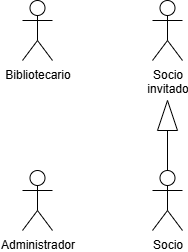
\includegraphics[scale=0.7]{imagenes/actores.png}
	\caption{Actores del sistema}
\end{figure}
En el diagrama se evidencia que el actor socio tendrá acceso a los mismos casos de uso que el socio invitado, pero sumando otros casos de uso propios.
\section{Requisitos de usuario}
Los requisitos de usuario reflejan las expectativas que tiene cada tipo de usuario a la hora de usar la aplicación; cómo espera que la misma se comporte cuando interactúa con ella, qué quiere encontrar... Estas necesidades de interacción y comportamiento del usuario a la aplicación se puede traducir en casos de uso.
\section{Casos de uso}
Ya definidos los actores que van a interactuar con el sistema, se procede a introducir los casos de uso.
Como introduce Francisco González \parencite{gonzalez2024casosuso} en los apuntes de su asignatura, un caso de uso representa una tarea o unidad coherente de funcionalidad que debe proporcionar el sistema a los actores, pudiendo participar varios actores diferentes en el mismo caso de uso. En este contexto, constituye una forma sencilla e intuitiva de documentar las funcionalidades que constituyen este sistema.
Se enumeran aquí los casos de uso desarrollados:
\begin{itemize}
	\item \textbf{CU01 -- Registrarse}
	\begin{itemize}
		\item \textbf{Actor:} Socio invitado.
		\item \textbf{Descripción:} Permite a un nuevo socio registrarse mediante un formulario, proporcionando datos como nombre, correo electrónico y contraseña. Si los datos son válidos, se crea el usuario y se inicia sesión automáticamente.
	\end{itemize}
	
	\item \textbf{CU02 -- Inicio de sesión}
	\begin{itemize}
		\item \textbf{Actor:} Bibliotecario, Administrador, Socio.
		\item \textbf{Descripción:} Permite a un socio acceder al sistema introduciendo sus credenciales. El sistema valida los datos y, en caso correcto, concede acceso según su rol (socio, bibliotecario o administrador).
	\end{itemize}
		
	\item \textbf{CU03 -- Recuperar contraseña}
	\begin{itemize}
		\item \textbf{Actor: Bibliotecario, Administrador, Socio.} 
		\item \textbf{Descripción: Mecanismo mediante el cual el usuario puede solicitar un enlace de recuperación de contraseña en caso de pérdida de la misma. Se envía un correo con este enlace, por lo que el usuario debe escribir el correo asociado a su cuenta para recibirlo.} 
	\end{itemize}
		
	\item \textbf{CU04 -- Consultar catálogo}
	\begin{itemize}
		\item \textbf{Actor:} Todos.
		\item \textbf{Descripción:} Permite buscar y visualizar los recursos disponibles en la biblioteca (obras y ejemplares). A partir de este caso de uso se pueden extender acciones como ver autores o ver ejemplares.
	\end{itemize}
	
	\item \textbf{CU05 -- Ver autores}
	\begin{itemize}
		\item \textbf{Actor:} Todos.
		\item \textbf{Descripción:} Permite consultar la información detallada de los autores asociados a las obras del catálogo. Extiende de la consulta de catálogo.
	\end{itemize}
	
	\item \textbf{CU06 -- Ver autor}
	\begin{itemize}
		\item \textbf{Actor:} Todos.
		\item \textbf{Descripción:} Permite consultar la información detallada de un autor determinado, como las obras pertenecientes a su autoría.
	\end{itemize}
	
	\item \textbf{CU07 -- Ver ejemplares}
	\begin{itemize}
		\item \textbf{Actor:} Todos.
		\item \textbf{Descripción:} Permite visualizar los ejemplares físicos concretos asociados a una obra, mostrando su estado y disponibilidad. Extiende de la consulta de catálogo.
	\end{itemize}
	
	\item \textbf{CU08 -- Consultar disponibilidad}
	\begin{itemize}
		\item \textbf{Actor:} Todos.
		\item \textbf{Descripción:} Permite comprobar si un ejemplar concreto se encuentra disponible para su préstamo o reserva en el momento de la consulta.
	\end{itemize}
	
	\item \textbf{CU09 -- Ver mi información personal}
	\begin{itemize}
		\item \textbf{Actor:} Administrador, Bibliotecario, Socio.
		\item \textbf{Descripción:} Permite al usuario acceder a los datos personales registrados en su perfil. A partir de esta vista se puede extender la modificación de los datos o la baja en el sistema, dependiendo del tipo de usuario.
	\end{itemize}
	
	\item \textbf{CU10 -- Modificar información personal}
	\begin{itemize}
		\item \textbf{Actor:} Administrador, Bibliotecario, Socio.
		\item \textbf{Descripción:} Permite al usuario actualizar sus datos personales (como dirección, correo o contraseña). Extiende de la visualización de la información personal. Algunos campos del formulario en el que consiste la vista del caso de uso cambia dependiendo del tipo de usuario.
	\end{itemize}
	
	\item \textbf{CU11 -- Darse de baja}
	\begin{itemize}
		\item \textbf{Actor:} Socio.
		\item \textbf{Descripción:} Permite al socio solicitar la eliminación o desactivación de su cuenta en el sistema. Extiende de la visualización de la información personal.
	\end{itemize}
	
	\item \textbf{CU12 -- Ver socios}
	\begin{itemize}
		\item \textbf{Actor:} Bibliotecario, Administrador.
		\item \textbf{Descripción:} Permite al usuario acceder al listado de todos los socios registrados en la biblioteca. A partir de esta vista se pueden extender las acciones de ver, modificar o eliminar un socio concreto.
	\end{itemize}
	
	\item \textbf{CU13 -- Ver socio}
	\begin{itemize}
		\item \textbf{Actor:} Bibliotecario, Administrador.
		\item \textbf{Descripción:} Permite visualizar la ficha detallada de un socio. Extiende del listado de socios.
	\end{itemize}
	
	\item \textbf{CU14 -- Modificar socio}
	\begin{itemize}
		\item \textbf{Actor:} Bibliotecario, Administrador.
		\item \textbf{Descripción:} Permite editar los datos de un socio registrado. Extiende de la visualización de un socio.
	\end{itemize}
	
	\item \textbf{CU15 -- Eliminar socio}
	\begin{itemize}
		\item \textbf{Actor:} Bibliotecario, Administrador.
		\item \textbf{Descripción:} Permite dar de baja a un socio del sistema. Extiende de la visualización de un socio.
	\end{itemize}
		
	\item \textbf{CU16 -- Modificación, visionado y borrado sobre bibliotecarios y administradores}
	\begin{itemize}
		\item \textbf{Actor:} Administrador.
		\item \textbf{Descripción:} Permite ver, modificar y eliminar bibliotecarios y administradores al administrador, extiende de ver usuarios.
	\end{itemize}
	
	\item \textbf{CU17-- Nuevo socio}
	\begin{itemize}
		\item \textbf{Actor:} Bibliotecario, Administrador.
		\item \textbf{Descripción:} Permite registrar manualmente a un nuevo socio en el sistema, recopilando sus datos personales.
	\end{itemize}
	
	\item \textbf{CU18 -- Gestionar catálogo / Registrar ejemplar}
	\begin{itemize}
		\item \textbf{Actor:} Bibliotecario, Administrador.
		\item \textbf{Descripción:} Permite dar de alta un nuevo ejemplar físico en el sistema. A partir de esta acción se pueden extender el registro de nuevos autores, editoriales o productoras.
	\end{itemize}
	
	\item \textbf{CU19 -- Registrar autor/editorial/productora}
	\begin{itemize}
		\item \textbf{Actor:} Bibliotecario, Administrador.
		\item \textbf{Descripción:} Permite añadir los datos de las entidades relacionadas con las obras (autores, editoriales o productoras) para poder vincularlas a los ejemplares. Extiende del registro de ejemplares.
	\end{itemize}
	
	\item \textbf{CU20 -- Duplicar ejemplar}
	\begin{itemize}
		\item \textbf{Actor:} Bibliotecario, Administrador.
		\item \textbf{Descripción:} Permite crear un nuevo registro de ejemplar tomando como base los datos de uno ya existente (por ejemplo, para añadir copias del mismo libro).
	\end{itemize}
	
	\item \textbf{CU21 -- Dar de alta bibliotecario}
	\begin{itemize}
		\item \textbf{Actor:} Administrador.
		\item \textbf{Descripción:} Permite al administrador registrar a un nuevo usuario con rol de bibliotecario, garantizando que solo personal autorizado tenga acceso a las funciones de gestión.
	\end{itemize}
	
	\item \textbf{CU22 -- CRUD sobre BBDD a través del panel de admin}
	\begin{itemize}
		\item \textbf{Actor:} Administrador.
		\item \textbf{Descripción:} Proporciona al administrador acceso total al panel de administración de Django para realizar operaciones de creación, lectura, actualización y borrado sobre cualquier registro del sistema.
	\end{itemize}
		
	\item \textbf{CU23 -- CRUD sobre todo tipo de usuarios}
	\begin{itemize}
		\item \textbf{Actor:} Administrador.
		\item \textbf{Descripción:} Permite al administrador gestionar de forma completa cualquier perfil de usuario del sistema (socios, bibliotecarios u otros administradores). Extiende del CRUD general sobre la base de datos.
	\end{itemize}
	
	\item \textbf{CU24 -- Prestar ejemplar a socio}
	\begin{itemize}
		\item \textbf{Actor:} Bibliotecario, Administrador.
		\item \textbf{Descripción:} Permite registrar el préstamo de un ejemplar a un socio. Incluye obligatoriamente la verificación de la disponibilidad del ejemplar.
	\end{itemize}
	
	\item \textbf{CU25 -- Devolver ejemplar}
	\begin{itemize}
		\item \textbf{Actor:} Bibliotecario, Administrador.
		\item \textbf{Descripción:} Permite registrar la devolución de un ejemplar prestado, actualizando su estado a disponible. Puede extenderse si el socio devuelve el ejemplar con retraso (aplicando penalización).
	\end{itemize}
	
	\item \textbf{CU26 -- Consultar mis préstamos}
	\begin{itemize}
		\item \textbf{Actor:} Socio.
		\item \textbf{Descripción:} Permite al socio consultar el estado de los préstamos que tiene activos. A partir de aquí puede extenderse la solicitud de prórroga.
	\end{itemize}
	
	\item \textbf{CU27 -- Consultar préstamos de socio}
	\begin{itemize}
		\item \textbf{Actor:} Bibliotecario, Administrador.
		\item \textbf{Descripción:} Permite al usuario consultar el historial y estado de los préstamos de un socio concreto.
	\end{itemize}
	
	
	\item \textbf{CU28 -- Solicitar prórroga}
	\begin{itemize}
		\item \textbf{Actor:} Administrador, Bibliotecario, Socio.
		\item \textbf{Descripción:} Permite al socio extender el plazo de devolución de un préstamo activo, siempre que se cumplan las condiciones establecidas. Extiende de la consulta de préstamos. El socio también puede solicitar esta acción a un bibliotecario, que tiene acceso a todos los préstamos de los socios.
	\end{itemize}

	\item \textbf{CU29 -- Ver préstamo}
	\begin{itemize}
		\item \textbf{Actor:} Bibliotecario.
		\item \textbf{Descripción:} Permite visualizar el detalle de un préstamo y prorrogar su fecha de devolución a petición del socio. Extiende de la consulta de préstamos de socio.
	\end{itemize}
	
\end{itemize}

Para dar una representación sencilla y visual de qué usuario desempeña cada caso de uso, se ha elaborado la tabla \ref{tab:relacion_cu_actores}, que lo muestra expresamente.
Adicionalmente, más adelante se puede encontrar un diagrama que ilustra la relación entre actores y casos de uso de una forma más visual. El lenguaje visual utilizado es \textit{UML (Unified Modeling Language)}, un estándar en la industria para modelar sistemas \textit{software} de todo tipo. Específicamente, se trata de un diagrama \textit{UML} de casos de uso, por lo que tiene sus propias reglas y elementos.
Este tipo de diagrama tiene como objetivo mostrar una vista genérica del funcionamiento del sistema elaborado a través de cómo se relacionan los actores con el mismo. Se pueden distinguir los siguientes elementos en el diagrama:

\begin{itemize}
	\item \textbf{Actores:} Representan los roles que adoptan las entidades externas (ya sean personas, sistemas hardware o software) que interactúan con la aplicación. Se representan gráficamente mediante monigotes y se sitúan fuera del límite del sistema. En el contexto de Liber, los actores principales son el Socio, el Bibliotecario y el Administrador (además del Socio invitado).
	
	\item \textbf{Sistema (o Límite del sistema):} Se representa mediante un rectángulo que engloba todos los casos de uso. Define las fronteras de la aplicación, es decir, qué funcionalidades pertenecen al sistema que se está modelando y cuáles son responsabilidad del entorno externo.
	
	\item \textbf{Casos de uso:} Son las funcionalidades o unidades de comportamiento que el sistema ofrece a sus actores. Se representan mediante elipses y su nombre suele ser una frase verbal (por ejemplo, ``Registrarse'', o ``Prestar ejemplar'').
	
	\item \textbf{Relaciones:} Son las líneas que conectan los elementos anteriores y definen cómo interactúan entre sí. Se distinguen tres tipos principales en este diagrama:
	\begin{itemize}
		\item \textbf{Asociación (Actor - Caso de uso):} Una línea continua que une un actor con un caso de uso, indicando que dicho actor interactúa con esa funcionalidad del sistema.
		\item \textbf{Inclusión (\texttt{<<include>>}):} Una flecha discontinua que apunta desde un caso de uso base hacia un caso de uso incluido. Se utiliza cuando un caso de uso contiene obligatoriamente el comportamiento de otro (por ejemplo, ``Prestar ejemplar'' incluye obligatoriamente ``Comprobar disponibilidad''). Evita duplicar comportamientos comunes.
		\item \textbf{Extensión (\texttt{<<extend>>}):} Una flecha discontinua que apunta desde un caso de uso de extensión hacia el caso de uso base. Se utiliza para indicar un comportamiento opcional o alternativo que solo ocurre bajo ciertas condiciones (por ejemplo, ``Renovar préstamo'' extiende de ``Consultar mis préstamos'', ya que no siempre se renueva).
	\end{itemize}
\end{itemize}
\begin{table}[H]
	\centering
	\caption{Relación de casos de uso y roles de usuario.}
	\label{tab:relacion_cu_actores}
	\small
	\begin{tabularx}{\textwidth}{X c c c c}
		\toprule
		\textbf{Caso de Uso} & \textbf{Invitado} & \textbf{Socio} & \textbf{Bibliotecario} & \textbf{Administrador} \\
		\midrule
		CU01 -- Registrarse & \checkmark & & & \\
		\addlinespace
		CU02 -- Inicio de sesión & & \checkmark & \checkmark & \checkmark \\
		\addlinespace
		CU03 -- Recuperar contraseña & & \checkmark & \checkmark & \checkmark \\
		\addlinespace
		CU04 -- Consultar catálogo & \checkmark & \checkmark & \checkmark & \checkmark \\
		\addlinespace
		CU05 -- Ver autores & \checkmark & \checkmark & \checkmark & \checkmark \\
		\addlinespace
		CU06 -- Ver autor & \checkmark & \checkmark & \checkmark & \checkmark \\
		\addlinespace
		CU07 -- Ver ejemplares & \checkmark & \checkmark & \checkmark & \checkmark \\
		\addlinespace
		CU08 -- Consultar disponibilidad & \checkmark & \checkmark & \checkmark & \checkmark \\
		\addlinespace
		CU09 -- Ver mi información personal & & \checkmark & \checkmark & \checkmark \\
		\addlinespace
		CU10 -- Modificar información personal & & \checkmark & \checkmark & \checkmark \\
		\addlinespace
		CU11 -- Darse de baja & & \checkmark & & \\
		\addlinespace
		CU12 -- Ver socios & & & \checkmark & \checkmark \\
		\addlinespace
		CU13 -- Ver socio & & & \checkmark & \checkmark \\
		\addlinespace
		CU14 -- Modificar socio & & & \checkmark & \checkmark \\
		\addlinespace
		CU15 -- Eliminar socio & & & \checkmark & \checkmark \\
		\addlinespace
		CU16 -- Modificación, visionado y borrado sobre bibliotecarios y administradores & & & & \checkmark \\
		\addlinespace
		CU17 -- Nuevo socio & & & \checkmark & \checkmark \\
		\addlinespace
		CU18 -- Gestionar catálogo / Registrar ejemplar & & & \checkmark & \checkmark \\
		\addlinespace
		CU19 -- Registrar autor/editorial/productora & & & \checkmark & \checkmark \\
		\addlinespace
		CU20 -- Duplicar ejemplar & & & \checkmark & \checkmark \\
		\addlinespace
		CU21 -- Dar de alta bibliotecario & & & & \checkmark \\
		\addlinespace
		CU22 -- CRUD sobre BBDD a través del panel de admin & & & & \checkmark \\
		\addlinespace
		CU23 -- CRUD sobre todo tipo de usuarios & & & & \checkmark \\
		\addlinespace
		CU24 -- Prestar ejemplar a socio & & & \checkmark & \checkmark \\
		\addlinespace
		CU25 -- Devolver ejemplar & & & \checkmark & \checkmark \\
		\addlinespace
		CU26 -- Consultar mis préstamos & & \checkmark & & \\
		\addlinespace
		CU27 -- Consultar préstamos de socio & & & \checkmark & \checkmark \\
		\addlinespace
		CU28 -- Solicitar prórroga & & \checkmark & \checkmark & \checkmark \\
		\addlinespace
		CU29 -- Ver préstamo & & & \checkmark & \\
		\bottomrule
	\end{tabularx}
\end{table}

\begin{figure}[H]
	\centering
	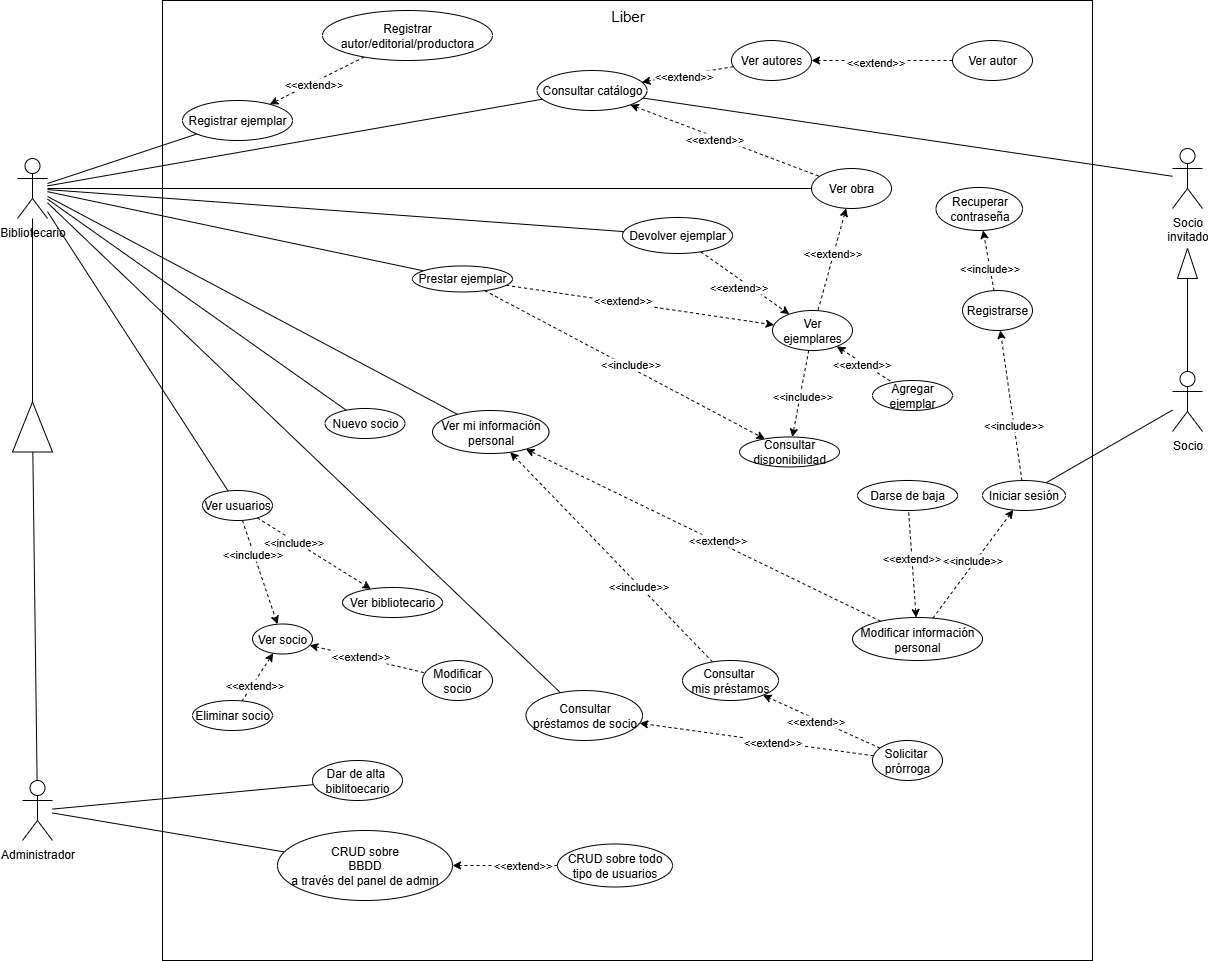
\includegraphics[width=\textwidth]{imagenes/casos_uso.png}
	\caption{Diagrama de casos de uso del sistema Liber.}
	\label{fig:diagrama_casos_uso}
\end{figure}

\section{Historias de usuario}

\section{Objetivos del trabajo}

Al estar tratando con proyecto de estas dimensiones, se hace necesaria una planificación estructurada a seguir para marcar tanto los plazos a cumplir como las restricciones y casos de uso específicos a tener en cuenta.	

\begin{table}[H]
	\centering
	\caption{Criterios de aceptación para el objetivo general OBJ-01.}
	\label{tab:criterios_aceptacion_normal01}
	\begin{tabularx}{\textwidth}{l X}
		\toprule
		\textbf{ID C.A.} & 
		\begin{minipage}[t]{\linewidth}
			\textbf{ID Objetivo asociado: OBJ-01} \\[2pt]
			\rule{\linewidth}{0.4pt} \\[2pt]
			\textbf{Descripción Criterio de Aceptación}
		\end{minipage} \\
		\midrule
		\textbf{CA-01} & El sistema debe permitir el alta, modificación, consulta y baja (CRUD) de Obras intelectuales, almacenando de forma obligatoria su título y signatura. \\
		\addlinespace
		\textbf{CA-02} & El sistema debe permitir la creación de Ejemplares físicos asociados obligatoriamente a una Obra preexistente, permitiendo marcar su estado de disponibilidad. \\
		\addlinespace
		\textbf{CA-03} & La aplicación debe gestionar correctamente la especialización de los ejemplares (Libros, Revistas, Periódicos y Grabaciones) cargando dinámicamente sus atributos específicos en la base de datos. \\
		\addlinespace
		\textbf{CA-04} & El catálogo debe soportar la relación de coautoría (relación N:M), permitiendo que una misma Obra sea vinculada a uno o varios Autores simultáneamente. \\
		\addlinespace
		\textbf{CA-05} & La interfaz del catálogo debe permitir a los usuarios realizar búsquedas funcionales y filtrados de los ejemplares empleando la interactividad en el frontal propia de Django. \\
		\addlinespace
		\textbf{CA-06} & El sistema debe validar a nivel de formulario y de base de datos que los identificadores estándar del catálogo (como el ISBN o el EAN) mantengan su propiedad de unicidad para garantizar la integridad de la información. \\
		\bottomrule
	\end{tabularx}
\end{table}

\begin{table}[H]
	\centering
	\caption{Criterios de aceptación para el objetivo general OBJ-02.}
	\label{tab:criterios_aceptacion_normal02}
	\begin{tabularx}{\textwidth}{l X}
		\toprule
		\textbf{ID C.A.} & 
		\begin{minipage}[t]{\linewidth}
			\textbf{ID Objetivo asociado: OBJ-02} \\[2pt]
			\rule{\linewidth}{0.4pt} \\[2pt]
			\textbf{Descripción Criterio de Aceptación}
		\end{minipage} \\
		\midrule
		\textbf{CA-01} & El sistema debe implementar un único modelo de base de datos centralizado para la entidad usuario que almacene obligatoriamente el nombre, los apellidos, una contraseña cifrada y un correo electrónico único que actúe como credencial de inicio de sesión. \\
		\addlinespace
		\textbf{CA-02} & El sistema debe permitir el acceso específico de los socios, validando que posean un número identificativo único y bloqueando automáticamente sus privilegios de reserva o préstamo en caso de que consten como penalizados en la base de datos. \\
		\addlinespace
		\textbf{CA-03} & La interfaz y los formularios para los bibliotecarios deben permitir, de manera exclusiva, la gestión ordinaria del catálogo y el registro de las transacciones de préstamo, validando su identidad mediante unas credenciales de acceso. \\
		\addlinespace
		\textbf{CA-04} & El rol de ADMINISTRADOR debe disponer de acceso total e irrestricto a través del panel de control de Django para realizar operaciones CRUD completas sobre cualquier tabla o registro de la infraestructura. \\
		\addlinespace
		\textbf{CA-05} & El backend debe denegar el acceso a rutas protegidas mediante un sistema de control de permisos (middleware), redirigiendo al usuario a la pantalla de inicio de sesión si intenta forzar manualmente URLs no autorizadas para su rol. \\
		\addlinespace
		\textbf{CA-06} & El sistema debe garantizar que las contraseñas de los usuarios nunca se almacenen en texto plano dentro de la base de datos PostgreSQL, delegando en el framework el cifrado automático mediante algoritmos de hash seguros. \\
		\bottomrule
	\end{tabularx}	
\end{table}

\begin{table}[H]
	\centering
	\caption{Criterios de aceptación para el objetivo general OBJ-3.}
	\label{tab:criterios_aceptacion_normal03}
	\begin{tabularx}{\textwidth}{l X}
		\toprule
		\textbf{ID C.A.} & 
		\begin{minipage}[t]{\linewidth}
			\textbf{ID Objetivo asociado: OBJ-3} \\[2pt]
			\rule{\linewidth}{0.4pt} \\[2pt]
			\textbf{Descripción Criterio de Aceptación}
		\end{minipage} \\
		\midrule
		\textbf{CA-01} & El sistema debe registrar automáticamente la transacción en la tabla de préstamos en el momento en que un bibliotecario la gestione, asignando la fecha actual a la fecha de inicio del préstamo. \\
		\addlinespace
		\textbf{CA-02} & La aplicación debe calcular de forma automática la fecha límite de devolución sumando el número de días estipulado por la política de la biblioteca a partir de la fecha de inicio de la transacción. \\
		\addlinespace
		\textbf{CA-03} & El sistema debe permitir la gestión de prórrogas antes de que termine el plazo del préstamo, verificando que el registro cuente con un número de prórrogas restantes mayor que cero, actualizando la fecha de la prórroga con la marca de tiempo actual y extendiendo la fecha de fin de manera proporcional. \\
		\addlinespace
		\textbf{CA-04} & Al solicitarse una prórroga válida, el backend debe descontar automáticamente en una unidad el contador de prórrogas disponibles para ese préstamo específico en la base de datos. \\
		\addlinespace
		\textbf{CA-05} & En el momento de la entrega física del recurso, el sistema debe registrar la fecha del día exacto en el campo de devolución. Si esta fecha es anterior o igual a la fecha límite, la transacción se considerará cerrada con éxito y el ejemplar volverá a estar disponible. \\
		\addlinespace
		\textbf{CA-06} & Si el sistema detecta que la devolución se realiza tarde (fecha de devolución posterior a la fecha límite), o que el plazo ha vencido sin haber devuelto el recurso, el backend debe activar de inmediato el estado de penalización del socio y registrar la fecha del bloqueo. \\
		\bottomrule
	\end{tabularx}	
\end{table}

\begin{table}[H]
	\centering
	\caption{Criterios de aceptación para el objetivo general OBJ-4.}
	\label{tab:criterios_aceptacion_normal04}
	\begin{tabularx}{\textwidth}{l X}
		\toprule
		\textbf{ID C.A.} & 
		\begin{minipage}[t]{\linewidth}
			\textbf{ID Objetivo asociado: OBJ-4} \\[2pt]
			\rule{\linewidth}{0.4pt} \\[2pt]
			\textbf{Descripción Criterio de Aceptación}
		\end{minipage} \\
		\midrule
		\textbf{CA-01} & El sistema debe disponer de un archivo Dockerfile en la parte backend que configure un entorno limpio basado en una imagen ligera de Python, instalando de forma automática todas las dependencias recolectadas en el archivo requirements.txt. \\
		\addlinespace
		\textbf{CA-02} & El entorno de la base de datos debe levantarse de forma aislada a través de un servicio independiente en el archivo docker-compose.yml, utilizando una imagen oficial y reciente de PostgreSQL. \\
		\addlinespace
		\textbf{CA-03} & El archivo docker-compose.yml debe orquestar la comunicación interna entre ambos contenedores (Django y PostgreSQL), garantizando que el contenedor web no intente arrancar hasta que el servicio de la base de datos esté completamente listo y operativo. \\
		\addlinespace
		\textbf{CA-04} & El contenedor de la base de datos debe implementar un volumen de Docker mapeado a la ruta de almacenamiento de PostgreSQL para asegurar la persistencia de los datos, impidiendo que el catálogo, los socios o los préstamos se borren al apagar o reiniciar los contenedores. \\
		\addlinespace
		\textbf{CA-05} & El sistema debe ser capaz de replicar exactamente el mismo comportamiento, rendimiento y configuración tanto al ser ejecutado en local (entorno de desarrollo) como al ser desplegado en plataformas en la nube sin necesidad de modificar el código fuente de la aplicación web. \\
		\bottomrule
	\end{tabularx}	
\end{table}

\begin{table}[H]
	\centering
	\caption{Criterios de aceptación para el objetivo general OBJ-5.}
	\label{tab:criterios_aceptacion_normal05}
	\begin{tabularx}{\textwidth}{l X}
		\toprule
		\textbf{ID C.A.} & 
		\begin{minipage}[t]{\linewidth}
			\textbf{ID Objetivo asociado: OBJ-5} \\[2pt]
			\rule{\linewidth}{0.4pt} \\[2pt]
			\textbf{Descripción Criterio de Aceptación}
		\end{minipage} \\
		\midrule
		\textbf{CA-01} & El proyecto debe incluir en su directorio raíz el archivo estandarizado LICENSE conteniendo el texto íntegro y oficial de la Licencia Pública General de GNU (GNU GPL v3), declarando formalmente el software como libre y abierto. \\
		\addlinespace
		\textbf{CA-02} & El código fuente de la aplicación Django debe subirse y estar disponible públicamente en una plataforma de control de versiones accesible (como GitHub o GitLab), permitiendo que cualquier usuario pueda clonar, bifurcar (fork) o descargar el repositorio sin restricciones. \\
		\addlinespace
		\textbf{CA-03} & Las vistas de Django, los modelos y las configuraciones de Docker deben contar con comentarios claros y documentación interna en las secciones complejas, simplificando la curva de aprendizaje para futuros miembros de la comunidad que deseen auditar o colaborar en el proyecto. \\
		\addlinespace
		\textbf{CA-04} & La configuración del sistema (como las claves secretas de Django o las credenciales de PostgreSQL) debe estar parametrizada mediante variables de entorno en un archivo .env.example, asegurando que cualquier usuario pueda desplegar su propia instancia de la biblioteca de forma local de manera inmediata y sin comprometer la seguridad. \\
		\bottomrule
	\end{tabularx}	
\end{table}

\begin{table}[H]
	\centering
	\caption{Criterios de aceptación para el objetivo general OBJ-6.}
	\label{tab:criterios_aceptacion_normal06}
	\begin{tabularx}{\textwidth}{l X}
		\toprule
		\textbf{ID C.A.} & 
		\begin{minipage}[t]{\linewidth}
			\textbf{ID Objetivo asociado: OBJ-6} \\[2pt]
			\rule{\linewidth}{0.4pt} \\[2pt]
			\textbf{Descripción Criterio de Aceptación}
		\end{minipage} \\
		\midrule
		\textbf{CA-01} & Demostrar la correcta aplicación de los fundamentos de ingeniería mediante el diseño e implementación del esquema lógico relacional en PostgreSQL, reflejando fielmente las restricciones de integridad y las relaciones de herencia. \\
		\addlinespace
		\textbf{CA-02} &  El desarrollo de la aplicación web debe evidenciar un desacoplamiento claro de responsabilidades siguiendo el patrón arquitectónico MVT (Modelo-Vista-Template) de Django, separando la lógica de acceso a datos de la lógica de presentación y de negocio. \\
		\textbf{CA-03} & La memoria del Trabajo de Fin de Grado debe documentar con rigor de ingeniería todas las fases del ciclo de vida del desarrollo de software, incluyendo el análisis de requisitos, el modelado formal (diagramas de casos de uso y de entidad-relación) y las pruebas de validación.  \\
		\addlinespace
		\bottomrule
	\end{tabularx}	
\end{table}

\section{Condiciones técnicas}

\section{Alcance y limitaciones}
	
	
	\printbibliography[heading=bibintoc, title={Bibliografía}]
\end{document}